% !TEX root = ../dissertation.tex

\chapter{Low Thrust Orbital Transfers using Reachability Sets}\label{sec:lowthrust_transfers}%

In this chapter, we propose a systematic design method which enables low-thrust transfers in the rotating frame of the \gls{rtbp} and \gls{rf2bp}.
The dynamics of a particle around an elongated small body can be modeled using the \gls{rf2bp} which are a slight reformulation of the relative dynamics presented in~\cref{sec:relative_eoms}.
There are many similarities between the well known \gls{rtbp} and \gls{rf2bp}.
In both mathematical models, there are are relative equilibirium points, also known as Lagrange points~\cite{szebehely1967,scheeres1994}, as well as periodic orbits around them.
As in the \gls{rtbp}, two of the equilibirum points around an elongated small body have an unstable saddle-center behavior and therefore the periodic orbits around these points also exhibit stable and unstable invariant manifolds~\cite{hu2002a,koon2011}.
The theory developed in the \gls{rtbp} is directly applicable to motion around asteroids~\cite{herrera2014}.

% why we need  low thrust transfers
The invariant manifolds of the \gls{rtbp} have been used previously to develop many low or energy free transfers~\cite{koon2000b,koon2001}.
In the case of the \gls{rtbp}, the invariant manifolds associated with the periodic orbits only pass close to the secondary body but do not pass near the primary body.
However, as a result it is not possible to directly utilize the invariant manifolds for orbital transfers for all scenarios, such as those departing from the primary body.
In the \gls{rf2bp} the invariant manifolds might approach or intersect the body depending on the shape or rotational rate. 
The manifolds of the \gls{rf2bp} offer additional opportunities for low energy transfers and can even be extended to landing or take off trajectories for sample return missions.

This chapter presents a low energy transfer scheme which leverages the use of low thrust propulsion to design transfer trajectories about the \gls{rtbp} and \gls{rf2bp}.
We utilize the concept of the reachability set to enable a simple methodology of selecting initial conditions to achieve general orbital transfers. 
The reachable set, defined as the set of all attainable states subject to the system constraints, allows for the extension of the previous control-free methods based on invariant manifolds.
Defining the reachable set on a \Poincare section reduces the dimensionality of the system dynamics to the study of a related discrete update map.
Through the use of low-thrust control input, the reachable set on the \Poincare section is enlarged and enables a larger space of potential transfers.

% low thrust inputs are accumulated (variational integrator)
The use of low thrust control inputs raises additional complications for numerical analysis.
kk
The method is formulated as an extension to the control free method based on invariant manifolds~\cite{koon2011}.
This paper provides a discrete optimal control formulation to generate the reachability set on a \Poincare section.

% outline of chapter
\section{Planar Circular Restricted Three Body Problem}\label{sec:pcrtbp}
% discuss some of the pros/cons of using PCRTBP model
We utilize the \gls{pcrtbp} as the basis of our system definition. 
It is a popular model in the preliminary analysis of multibody spacecraft trajectories. 
In the context of Earth based mission, the \gls{pcrtbp} affords a relatively simple dynamic model while still capturing the major third body perturbation of the Moon.
In addition, this model allows for a systematic process to define and exploit \Poincare sections.
Furthermore, the 2D solutions afforded by the \gls{pcrtbp} are frequently used to gain a qualitative understanding of the trade space of transfers in the Earth-Moon system.
The PCRTBP approach offers insight into the fundamental dynamical structure while capturing the major dynamic properties of the planar motion.
As a result, this approach is best suited for preliminary trajectories which do not require large plane changes.

The Earth is assumed to be the more massive primary, \( m_1 \), while the Moon is the second, smaller primary \( m_2\).
The equations of motion are developed in a rotating reference frame which allows for much greater insight into the structure of the dynamics.
This rotating reference frame is later used when deriving the motion about an asteroid.
Following convention, the system is also non-dimensionalized by the characteristic units of length, mass, and time~\cite{koon2011}.
As a result, the system can be characterized by a single mass ratio parameter \( \mu \),
\begin{equation}
        \mu = \frac{m_2}{m_1+m_2} \, .
        \label{eq:mass_param}
\end{equation}
In the rotating reference frame the Lagrangian is given by
\begin{equation}\label{eq:pcrtb_lagrangian}
    L = \frac{1}{2} \parenth{\parenth{\dot{x} - y}^2 + \parenth{\dot{y} + x}^2} + \frac{1 - \mu}{r_1} + \frac{\mu}{r_2},
\end{equation}
where the distances \( r_1, r_2 \in \R \) define the distance from the spacecraft to each primary and are defined as
\begin{align}
    r_1 &= \sqrt{\parenth{x + \mu}^2 + y^2} , \\
    r_2 &= \sqrt{\parenth{x -1 + \mu}^2 + y^2} .
\end{align}
Following a straightforward application of the Euler-Lagrange equations, a more detailed derivation is provided in~\cite{szebehely1967}, results in the following equations of motion defined in the rotating reference frame
\begin{equation}\label{eqn:cont_dyn}
        \left[\begin{array}{c} \dot{\vc{r}} \\ \dot{\vc{v}} \end{array} \right] = 
        \left[ \begin{array}{c} \vc{v} \\ A \vc{v} + \nabla U + \vc{u} \end{array} \right] = f\left( t,\vc{x}, \vc{u}\right) \, ,
\end{equation}
where the matrix \( A \) and pseudo gravitational potential gradient \( \nabla U\) are
\begin{align}
    A &= \left[ \begin{array}{ccc} 0 & 2 & 0 \\ -2 & 0 & 0 \\ 0 & 0 & 0 \end{array} \right], \label{eq:A_mat} \\
    \nabla U &= \left[ \begin{array}{c} x - \frac{ \left(1 - \mu\right) \left(x + \mu\right)}{r_1^3} - \frac{\mu \left( x - 1 + \mu \right)}{r_2^3} \\
                                                                                        y - \frac{ \left(1 - \mu\right) y}{r_1^3} - \frac{\mu y}{r_2^3} \\
                                                                                        - \frac{ \left(1 - \mu\right) z}{r_1^3} - \frac{\mu z}{r_2^3}\end{array}\right]
                                        = \left[\begin{array}{c} U_x \\ U_y \\ U_z\end{array} \right] , \label{eq:grav_pot}
\end{align}
and the control input is defined as \( \vc{u} = \begin{bmatrix} u_x & u_y \end{bmatrix}^T \in \R^{2\times1} \) and assumed to be continuously variable but bounded in magnitude, i.e. \( \vc{u}^T \vc{u} \leq u_{max}^2 \).
The state is defined as \( \vc{x} = \begin{bmatrix}\vc{r} &\vc{v} \end{bmatrix}^T\) with \(\vc{r} = \begin{bmatrix} x & y \end{bmatrix}^T \in \R^{2\times1}\) and \(\vc{v}= \begin{bmatrix} \dot{x} & \dot{y} \end{bmatrix}^T \in \R^{2\times1}\) representing the position and velocity with respect to the system barycenter, respectively.

\subsection{Jacobi Integral}\label{sec:jacobi}
There exists a single integral, or constant of motion for the three-body problem~\cite{szebehely1967,lanczos1970}.
This energy constant is analogous to the total mechanical energy, however it is a non-physical quantity arising from the problem formulation~\cite{szebehely1967}.
Also known as the Jacobi constant, it is defined as a function of the position and velocity in the rotating frame and given by
\begin{equation}
        E\left( \vc{r} , \vc{v} \right) = \frac{1}{2}\left( \dot{x}^2 + \dot{y}^2\right) - U\left(x,y \right) \, .
        \label{eq:jacobi}
\end{equation}
\Cref{eq:jacobi} divides the phase space into distinct regions of allowable motion based on the energy level of the spacecraft.
Fixing the Jacobi integral to a constant defines zero velocity curves, which are the locus of points where the kinetic energy, and hence velocity vanishes.
As seen in Figure~\ref{fig:energy_contour}, the phase space is divided into distinct realms based on the energy level.
In the vicinity of \( m_1\) or \(m_2\) there exists a potential well. 
As the energy level increases there are five critical points of the effective potential where the slope is zero.
Three collinear saddle points on the \(\hat{e}_1\) axis and two equilateral points.
These equilibrium, or Lagrange points, are labeled \( L_i, i = 1, \hdots, 5 \) and are shown in Figure~\ref{fig:energy_contour}.
The Jacobi integral is a valuable invariant property of the three-body system that allows for greater insight into the motion of the spacecraft.
\begin{figure}[htbp]
        \centering
        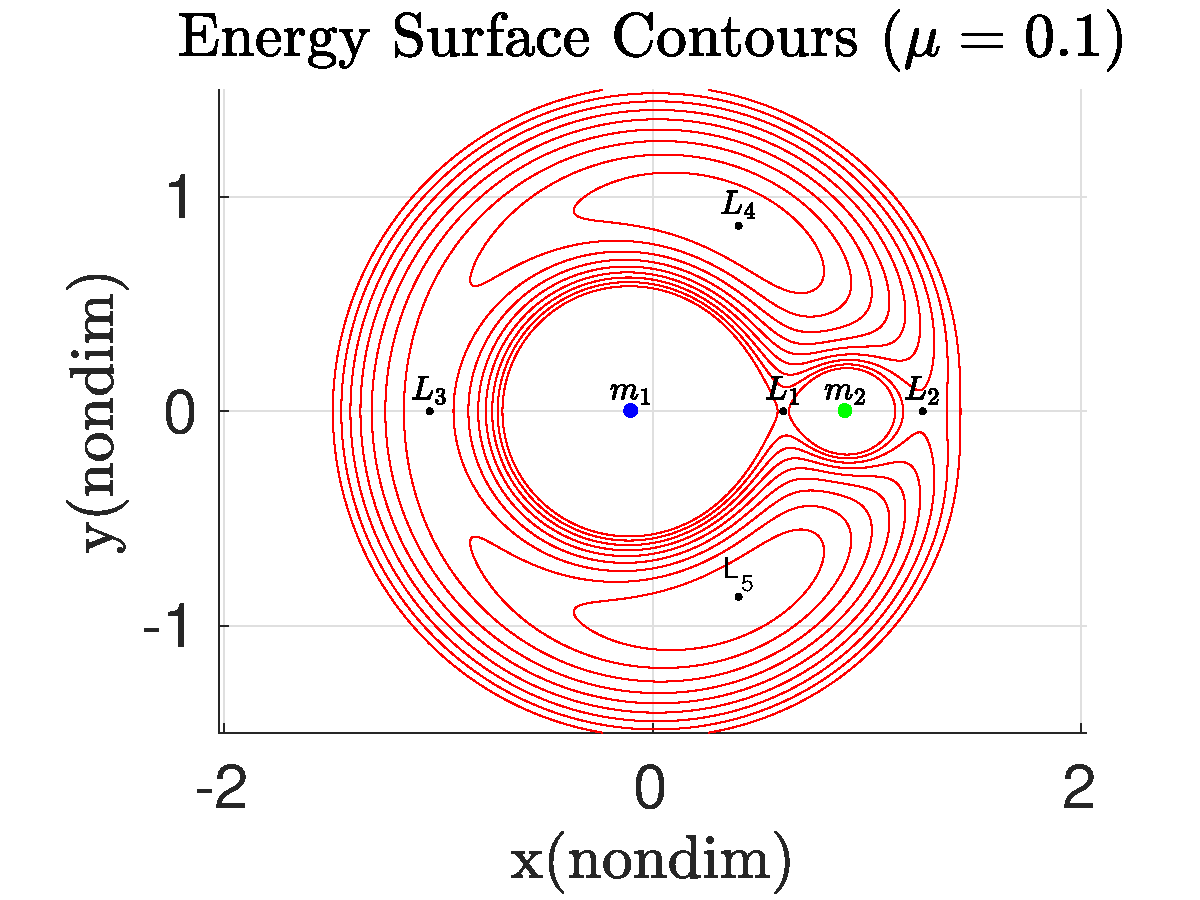
\includegraphics[width=0.75\textwidth]{./figures/2017_JAS/energy_contours.pdf}
        \caption[Jacobi integral]{Contour plot of Jacobi integral: Zero velocity curves of constant Jacobi integral. A particle with fixed energy level cannot cross the contour lines and is therefore limited to specific regions of the phase space. }
        \label{fig:energy_contour}
\end{figure} 

\subsubsection{Invariant Manifolds and \Poincare Map}\label{sec:invariant_manifold}
Dynamics systems theory has been applied to the design of control-free maneuvers in the restricted three-body problem~\cite{koon2011}.
As previously introduced in~\Cref{sec:jacobi}, there exist five equilibrium points in the equations of motion for the three-body problem.
It has been shown that the local orbit structure near the Lagrange points gives rise to families of periodic orbits as well as the stable and unstable manifolds of these periodic orbits.
This rich structure is globally connected and gives rise to a dynamical chain which allows trajectories to pass through the phase space~\cite{koon2011,conley1968}.
The manifold structure associated with periodic orbits about the \( L_1 \) and \( L_2 \) Lagrange points are critical to the understanding of the motion of spacecraft as well as comets/asteroids.
In addition, the stable and unstable manifolds serve as the boundaries of the phase space region that allow for the transport between realms in a single three-body system or between multiple three-body systems.
These invariant manifolds only exist as a result of the dynamic formulation of the three-body problem in a rotating reference frame. 
Invariant manifolds serve as a higher dimensional generalization of the concept of seperatrices from linear systems as applied to the case of nonlinear systems. 

\Poincare maps are a useful tool in the analysis of the flow near periodic orbits in the three-body problem.
We let \( \Sigma \) define a hypersurface of section chosen such that all trajectories in the vicinity of a state \( \vc{q} \in \Sigma \) cross \( \Sigma \) transversely and in the same direction.
A \Poincare map, \( P(\vc{q}) = \phi(T;\vc{q}) \), maps the state of a trajectory from one intersection to the next.
Choosing a section in this manner results in a \Poincare section as shown in~\cref{fig:poincare_map}.
In~\cref{fig:poincare_map} we show two examples of periodic trajectories intersecting the \Poincare section. 
Periodic solutions will appear as fixed points on the section, such as \( q_0, q_1 \) in~\cref{fig:poincare_map}, while stable or unstable trajectories become clearly visible by viewing successive intersections of the section.
This allows for greater insight into the stability and dynamics of periodic solutions of a dynamic system as a fixed point on the \Poincare section corresponds to a periodic orbit while movement on the section is associate with the stability of neighboring trajectories. 
For example, \Poincare maps have been used to prove the existence of homoclinic orbits, which are orbits both forward and backward asymptotic to a single unstable periodic orbit, and heteroclinic orbits, which join different periodic orbits~\cite{conley1968,koon2000b}.
These dynamic features have been shown to play a vital role in the movement of natural bodies as well as critical for spacecraft missions~\cite{gomez2001,lo1997}.

\begin{figure}
    \centering
    \includegraphics[width=\textwidth,height=0.1\textheight]{tikz/poincare_map.tikz}
    \caption{Diagram of the \Poincare map: Periodic orbits will appear as fixed points on the \Poincare section \( \Sigma \). Stability of periodic orbits is clearly visible on the section as successive intersections approach or depart a fixed point.\label{fig:poincare_map}}
\end{figure}
% drawbacks of this approach on how we seek to improve upon it
Combining invariant manifolds and an appropriate \Poincare section provides a conceptually simple manner to determine trajectories which connect wide regions of the phase space.
However, the results previously developed are highly case specific and difficult to generalize to arbitrary transfers.
Also, these results are based on control-free trajectories which rely on the underlying structure of the three-body system.
In addition, transfer orbits along an invariant manifold require large time of flights which may be undesirable for time critical missions.
The addition of low-thrust propulsion offers the potential of reduced transit times and the ability to depart from the free motion trajectory to allow for increased transfer opportunities. 
In this paper, we formulate an optimal control problem to generate the reachable set of the spacecraft.
We compute the reachable set on an appropriate \Poincare section and use this to design a transfer trajectory.

% TODO Generalize this description to be applicable to both the PCRTBP and Asteroid examples

\section{Transfer Design around Asteroids}\label{sec:sc_eoms}

The motion of a massless particle, or spacecraft, about an asteroid shares many similarities with that of the three-body problem.
As is typical in the three-body problem, the equations of motion are usually represented in a uniformly rotating frame aligned with the two primaries.
Similarly, the equations of motion about an asteroid are also defined in a body-fixed frame with uniform rotation.
In this reference frame, the gravitational potential field is time invariant and only a function of the position of the particle.
In addition, since the rotational rate of the asteroid is constant, the equations of motion are time invariant.
Finally, the use of the rotating reference frame allows for much greater insight into the dynamic structure of the behavior around the asteroid.
Here we consider a simplified form of the relative equations of motion about an asteroid.
We only treat the translational motion of the spacecraft with respect to the asteroid instead of the full coupled equations of motion introduced in~\cref{sec:asteroid_dumbbell_eoms}.

We define a reference frame originating at the center of mass of the asteroid.
The body-fixed reference frame is composed of the unit vectors \( \hat{\vc{x}} , \hat{\vc{y}}, \hat{\vc{z}} \), which are aligned along the principal axes of smallest, intermediate, and largest moment of inertia, respectively.
The body-fixed equations of motion of a massless particle about an arbitrarily rotating asteroid are given by
\begin{align}\label{eq:body_eoms}
    \ddot{\vc{r}} + 2 \vc{\Omega} \times \dot{\vc{r}} + \vc{\Omega} \times \parenth{ \vc{\Omega} \times \vc{r} } + \dot{\vc{\Omega}} \times \vc{r} = \nabla U(\vc{r}) ,
\end{align}
where \( \vc{\Omega} \in \R^{3 \times 1}\) is the instantaneous angular velocity vector of the asteroid represented in the body-fixed frame, \( \vc{r} \) is the position of the particle in the body-fixed frame, and \( \nabla U(\vc{r}) \) is the gradient of the gravitational potential~\cite{scheeres2012a}.
We assume that the asteroid rotates at a uniform rate, \( \norm{\vc{\Omega}} = \omega \in \R^1 \), about the axis of the maximum moment of inertia, i.e.\ \( \vc{\Omega} = \omega \hat{\vc{z} }\).
As a result, we can represent the equations of motion in scalar form as
\begin{align} \label{eq:eoms}
    \begin{split}
        \ddot{x} - 2 \omega \dot{y} - \omega^2 y &= U_x , \\
        \ddot{y} + 2 \omega \dot{x} - \omega^2 x &= U_y , \\
        \ddot{z} &= U_z .
    \end{split}
\end{align}

In this situation, the state is defined as \( \vc{x} = \bracket{\vc{r}~\>\vc{v}}^T \in \R^{6 \times 1}\) with \(\vc{r} = \bracket{x~\>y~\>z}^T \in \R^{3\times1}\) and \(\vc{v}= \bracket{ \dot{x}~\>\dot{y}~\>\dot{z} }^T \in \R^{3\times1}\) representing the position and velocity with respect to the body-fixed frame, respectively.
We further assume that our spacecraft is capable of exerting a translational acceleration, \( \vc{u} \in \R^{3\times1} \), in any direction, while subject to a maximum magnitude constraint, \( \norm{\vc{u}} \leq u_m \).
This is typical of many spacecraft which offer full rotational freedom and can direct a potentially varying force or acceleration in any direction.
The equations of motion may be rewritten in state space form as
\begin{align}\label{eq:state_space_eoms}
    \begin{bmatrix} \dot{\vc{r}} \\ \dot{\vc{v}} \end{bmatrix} &=
    \begin{bmatrix}\vc{v} \\ \vc{g} \parenth{\vc{r}} + \vc{h}\parenth{\vc{v}} + \vc{u} \end{bmatrix} ,
\end{align}
where the terms \(\vc{g} \parenth{\vc{r}} \) and \( \vc{h}\parenth{\vc{v}} \) are given by
\begin{align}\label{eq:state_space_terms}
    \vc{g}\parenth{\vc{r}} = \begin{bmatrix}  U_x + \omega^2 x \\ U_y + \omega^2 y \\ U_z \end{bmatrix} ,\quad
    \vc{h}\parenth{\vc{r}} = \begin{bmatrix} 2 \omega \dot{y} \\ -2 \omega \dot{x} \\ 0 \end{bmatrix} .
\end{align}

Since Castalia is a uniformly rotating asteroid, the equations of motion are time invariant when represented in the body-fixed frame.
In addition, there exists an integral of motion, or a conserved quantity, that is constant for all motion of a particle.
The Jacobi constant, \( J (\vc{r} , \vc{v} ) \), is given by
\begin{align}\label{eq:jacobi}
    J \parenth{\vc{r}, \vc{v}} = \frac{1}{2} \omega^2 \parenth{x^2 + y^2} + U(\vc{r}) - \frac{1}{2} \parenth{\dot{x}^2 + \dot{y}^2 + \dot{z}^2} .
\end{align}
The Jacobi constant functions in a similar manner as used in three-body problem~\cite{szebehely1967}.
We can define zero-velocity surfaces using the Jacobi constant by fixing the value to a desired constant.
The zero-velocity surfaces are the locus of points where the kinetic energy and hence velocity vanishes.
Just as in the three-body problem, the Jacobi constant in~\cref{eq:jacobi} divides the phase space into distinct realms of possible motion.
Similarly, there exist, in general, four equilibrium points and also their associated stable and unstable manifolds~\cite{scheeres1996,scheeres1994}.
The properties of these manifolds play a critical role in the dynamics of trajectories in their vicinity.

\section{Optimal Control Formulation for Reachability Set}\label{sec:optimal_control}
% introduce method
In this section, an optimal control formulation is presented to determine and design transfers within the three-body problem.
The application of variational integrators to optimal control problems is referred to as computational geometric optimal control.
Our formulation is based on the concept of the reachability set on a \Poincare section.
This method allows one to easily determine potential transfer opportunities by finding set intersections on a lower dimensional space and greatly reduces the design process.
The addition of continuous low thrust propulsion extends the control free design process developed previously and allows for a greater range of potential transfers with a reduced time of flight.

The numerical examples presented in this section are designed in the context of the PCRTBP.
The dynamic environment has a four dimensional state space and offers a convenient integration constant in the form of the Jacobi integral.
As a result, there are well defined methods to define and exploit \Poincare sections, which result in straightforward two-dimensional subspaces of the system.
Our approach uses the \Poincare section to approximate the reachability set on this reduced subspace.
As a result, this approach is more difficult to apply to three-dimensional transfers in the general three body problem.
\Poincare sections in the case of the general six dimensional state space are significantly more challenging and typically require more complicated visualization techniques. 
However, this is an area of active research and some of the authors future research is aimed at implementing this approach for non-planar transfer trajectories~\cite{kulumani2016d}.

\subsection{Reachability Set}\label{sec:reachability_set}
% discuss reachability and application to space system
Reachability theory provides a framework to evaluate control capability and safety.  
The reachable set contains all possible trajectories that are achievable over a fixed time horizon from a defined initial condition, subject to the operational constraints of the system.
Reachability theory has been applied to aerospace systems such as collision avoidance, safety planning, and performance characterization.
The theory formally supporting reachability has been extensively developed and is directly derivable from optimal control theory~\cite{varaiya2000,lygeros2002,lygeros2004}.
More recently, reachability theory has recently been applied to space systems~\cite{holzinger2009,komendera2012a,dellnitz2006}.
Computation of the reachable set for a system involves solving the Hamilton-Jacobi partial differential equation or satisfying a dynamic programming principle.
Analytical computation of reachable sets is an ongoing problem and is only possible for certain classes of systems.
Typically, numerical methods are used to generate approximations of the reachability set, but are generally limited by the dimensionality of the problem.
 
Computation of reachable sets is critical to space situational awareness, rendezvous and proximity operations, and orbit determination operations.
Specifically, maintaining accurate estimates of a spacecraft state over extended periods is not trivial.
The challenge is increased for multiple spacecraft operating in close proximity or when there are long periods of time between measurements.
Coupling the ability for continuous low-thrust propulsion between measurements increases the measurement association complexity.
Computing the reachability set given estimated states and control authorities allows one to better correlate subsequent measurements or determine sensor pointing regions in the event of a lost spacecraft. 


\subsection{Optimal Control Formulation}\label{sec:optimal_control}
In this paper, we seek to approximate the reachability set on a \Poincare section by solving a related optimal control problem. 
We choose our \Poincare section in a similar manner to those used previously for the design of transfers via invariant manifolds.
The \Poincare section is chosen to intersect transversally with trajectories emanating from the initial orbit. 
In the case of a periodic orbit the trajectories will cross the \Poincare section at two distinct fixed points every half period.
The main idea is that the addition of low thrust propulsion allows us to enlarge the set of trajectories achievable in the \Poincare section. 
\Cref{fig:reachability_set} illustrates how, without any control input, trajectories will intersect with the \Poincare section at \( \vecbf{x}_n \). 
However, the addition of low thrust propulsion allows the spacecraft to depart from the natural dynamics and intersect the \Poincare section at a different location.
We use a cost function to define a distance metric on the \Poincare section from the control-free intersection to an intersection under the influence of the control input.
Maximization of this distance along varying directions enables us to generate the largest reachability set under the bounded control input.
In~\cref{fig:reachability_set} the reachable set is shown as a circular region on the \Poincare section.
In practice, the reachable set will be of a general shape and also higher dimensional in the nonplanar case.
\begin{figure}
        \centering
        \includegraphics[width=\textwidth]{tikz/reachability_set.tikz}
        \caption{Reachability set on a \Poincare section: Pictorial representation of the reachability set (blue circle) on the \Poincare section, \(\Sigma\). 
            The terminal state, \( x_n\), is the intersection without any control input. 
            Adding a control input allows for the terminal state, \( x_f \), to be displaced by some distance/cost \( J \) as measured on the section.
            We parameterize a specific direction on the section with the angles \( \theta_d\) and seek to maximize the distance between \( x_f \) and \( x_n \).
            Computation of the maximum distance, or reachability, for a variety angles gives a discrete approximation of the reachability set.\label{fig:reachability_set}}
\end{figure}

We define the \Poincare section along the horizontal axis, which is equivalent to the surface \( y = 0 \), and given by
\begin{align}
        \Sigma = \braces{ ( x, \dot{x}) \, | \, y = 0} . 
        \label{eqn:poincare_section}
\end{align}
This is similar to the previous work in determining homoclinic orbits in the three-body problem~\cite{llibre1985,koon2011}.
Previous analytical results have shown that homoclinic orbits intersect transversally in the \( (x, \dot{x} ) \) space on the plane \( y = 0 \).
We seek to compliment these results with the addition of low thrust propulsion to maximize the reachable set on the \Poincare section.
Placing our section at \( y = 0\) ensures that all trajectories will intersect our section.
An optimal control problem is defined by a  cost function
\begin{equation}
        J = -\frac{1}{2} \left( \vc{x}(N) - \vc{x}_{n}(N)\right)^T 
        \left[
        \begin{array}{cccc}
                1 & 0& 0& 0 \\
                 0& 0& 0& 0\\
                 0 & 0 & 1 &0\\
                 0 & 0& 0& 0
        \end{array}
        \right]
        \left( \vc{x}(N) - \vc{x}_{n}(N)\right) = \phi(\vc{x}(N),\vc{x}_n(N)) \, .
        \label{eq:cost}
\end{equation}
The term \( \vc{x}_n(N) \) is the final state of a control-free trajectory while the term \( \vc{x}(N)\) is the final state under the influence of the control input.
Maximization of the distance between \( \vc{x}_n \) and \(\vc{x} \), on the \Poincare section defined in~\cref{eqn:poincare_section} at the terminal time \( t_f = N \), is equivalent to the minimization of \( J \) defined in~\cref{eq:cost}.
The \Poincare section is defined through the use of appropriate terminal constraints given by
\begin{subequations}
\begin{align}
    v_1( \vc{x}(N) ) &= y(N) = 0 \, , \\ 
    v_2 ( \vc{x}(N) )&=  \frac{\dot{x}(N) - \dot{x}_n(N) }{x(N) -x_n(N) } - \tan{\theta_d} = 0\, , \\
         0 &\geq\vc{u}^T \vc{u} - u_{max}^2 \, ,
\end{align}
    \label{eq:constraints}
\end{subequations}
where the angle \( \theta_d\) defines a direction in which we wish to maximize the reachability set on the \Poincare section.
The maximum control thrust magnitude is defined by \( u_{max} \) and is non-dimensionalized by the characteristic units of length, mass, and time.
The goal is to determine the control input \( \vc{u}_k\) such that the cost function~\cref{eq:cost} is minimized subject to the state equations of motion~\cref{eqn:cont_dyn} and constraints~\cref{eq:constraints}.

Application of the Euler-Lagrange equations allows us to derive the necessary conditions for optimality~\cite{bryson1975}.
This results in an optimal control problem and the necessary conditions are given as
\begin{subequations}\label{eq:necc_cond}
\begin{align}
    \dot{\vc{\lambda}} &= - \deriv{H}{\vc{x}}, \\
        0 &=  \deriv{H}{\vc{u}} \, , \label{eqn:control_necc_cond}\\
        0 &= \deriv{\phi}{\vc{x}}^T + \deriv{\vc{v}}{\vc{x}}^T \vc{\beta}  - \vc{\lambda}^T(N) \, ,  
\end{align}
\end{subequations}
where the Hamiltonian \(H\) is defined as
\begin{equation}
        H = \vc{\lambda}^T \vc{f}(\vc{x}, \vc{u}) \, ,
        \label{eq:hamiltonian_opt}
\end{equation}
and \( \vc{\lambda} \in \R^{4 \times 1} \) is the costate and \(\vecbf{\beta} \in \R^{2 \times 1} \) are the additional Lagrange multipliers associated with the terminal constraints in~\cref{eq:constraints}.
The state dynamics are represented by \( \vc{f}(\vc{x}_k, \vc{\lambda}_k ) \) after substituting~\cref{eqn:control_necc_cond} into~\cref{eqn:cont_dyn}.
This indirect optimal control formulation leads to a two point boundary value problem with split boundary conditions. 
By sweeping the angle \( \theta_d \) one can approximate the reachable set on the \Poincare section subject to the bounded control input. 

The optimal control formulation presented in this section results in a \gls{tpbvp}. 
There exist many methods to solve \glspl{tpbvp} such as gradient, quasilinearization, and shooting methods~\cite{bryson1975,kirk2012}.
Shooting methods are common in astrodynamic trajectory design problems and relatively simple to implement.
In the shooting method, initial conditions are varied such that a terminal constraint is satisfied, similar to the way an archer modifies the bow in order to more accurately strike a target. 
Consider the vector of initial conditions, \( \vc{\chi} = \braces{\vc{x}_0, \vc{\lambda}_0}\), which is varied to satisfy some terminal constraints of the form \( \vc{G}(\vc{\chi}) = \braces{\vc{x}_t - \vc{x}_n} = 0 \).
The free variables at the terminal time are computed by propagation of \( \vc{\chi} \) over the selected time horizon. 
At the terminal time, the constraint vector is calculated and if not satisfied \( \vc{\chi}\) is varied.
Rather than numerical integration over the entire time interval, multiple shooting segments the interval into several smaller sub-arcs~\cite{stoer2013}.
This multiple shooting approach incorporates additional interior constraints but reduces the sensitivity of the costates along each sub-arc.
The use of the multiple shooting method reduces the sensitivity of changes in the initial costate at the expense of additional design variables, but has been shown to provide more stable and robust solutions~\cite{ozimek2010a}.

\begin{figure}
    \centering
    \includegraphics[width=\textwidth]{tikz/multiple_shooting.tikz}
    \caption{Schematic diagram of the multiple shooting method:
        The complete trajectory is split into a number of sub-segments, and additional interior constraints are included to ensure state and costate continuity.
        Splitting the optimal trajectory into short segments reduces the sensitivity of terminal states to variations of the initial states.\label{fig:multiple shooting}}
\end{figure}

In~\cref{fig:multiple shooting}, we show a schematic representation of the multiple shooting procedure.
We split the optimal control horizon into equal length subsegments such that the length of each segment is \( \frac{k}{n} \), where \( k, n \) are the total number of steps and number of stages, respectively.
Similarly, we divide the state and costate trajectories into \( n \) equal segments. 
To ensure continuity, additional interior constraints are incorporated as
\begin{align}\label{eq:interior_constraints}
        \vc{x}_1^{-} - \vc{x}_1^{+} &= 0 , \nonumber\\ 
        \vc{\lambda}_1^{-} - \vc{\lambda}_1^{+} &= 0 , \nonumber\\
        \vc{x}_2^{-} - \vc{x}_2^{+} &= 0 , \nonumber\\ 
        \vc{\lambda}_2^{-} - \vc{\lambda}_2^{+} &= 0 , \nonumber\\
        &\vdots \nonumber \nonumber\\
        \vc{x}_{n-1}^{-} - \vc{x}_{n-1}^{+} &= 0 , \nonumber\\ 
        \vc{\lambda}_{n-1}^{-} - \vc{\lambda}_{n-1}^{+} &= 0.
\end{align}
Using the multiple shooting method reduces the sensitivity of the terminal states, \( \vc{x}_i^{+}, \vc{\lambda}_i^{+}\), to variations of the initial states, \(\vc{x}_{i-1}^{-}, \vc{\lambda}_{i-1}^{-}\).
As a result, the design vector \( \vc{\chi} \) is augmented with the additional interior initial conditions, \( \vc{x}_i^{-}, \vc{\lambda}^{-}\).
Similarly, the constraint vector is augmented with the additional interior constraints defined in~\cref{eq:interior_constraints}.
Based on experimentation, we use four stages in our multiple shooting method.
This provided the best performance and convergence stability while minimizing the difficulties in additional interior constraints.
The multiple shooting algorithm now varies the design vector \( \vc{\chi}\) to ensure that the constraints in \( \vc{G}(\vc{\chi}) \) are satisfied.
In this work, we use the Matlab nonlinear solver \texttt{fsolve} to solve the system of nonlinear equations defined by the multiple shooting algorithm with a convergence tolerance of \num{1e-5}.
Within \texttt{fsolve}, we use the trust-region dogleg solver which makes use of the Powell dogleg procedure for computing a step direction and magnitude to minimize successive iterations of the solver.
The numerical results are specific to the choice of nonlinear solver, and different tolerances or software tools may result in slight changes.

% TODO Add numerical examples of the three-body problem
\section{Numerical Examples of Transfers using Reachability Sets}\label{sec:simulation}
We present two numerical simulations in the Earth-Moon system to demonstrate the transfer procedure.
These simulations enable the spacecraft to depart from the natural dynamics through the use of low-thrust propulsion.
The reachability set on the \Poincare section allows for a straightforward method of determining transfer opportunities.
The first example is a transfer from a periodic orbit of the \( L_1 \) Lagrange point to a fixed orbit of the moon.
This example uses a single iteration of the reachable set computation in the design of the transfer.
The second example is a transfer from geostationary orbit of the Earth to a period orbit of \( L_1 \). 
This examples demonstrates the ability to extend the reachability process to multiple iterations, to allow for a much larger and more general transfer.
With both examples it is possible to depart from the vicinity of the Earth to a Moon orbit via a series of reachable sets defined on \Poincare sections.
The numerical examples presented in this section satisfy the necessary conditions for local optimality and obtaining a globally optimal solution is considered beyond the scope of this paper.
Next, the results are extended from the planar problem to three dimensions with a simulation about asteroid 4769 Castlia.
This numerical examples demonstrates the extension of the method to the more complicated dynamic enviornment around an asteroid.

\subsection{Three Body Examples}

\paragraph{Periodic Orbit Transfer}\label{sec:periodic_orbit_transfer}
The first objective is to design a transfer trajectory from a planar periodic orbit about the \( L_1\) Lagrange point to a bounded orbit in the vicinity of the Moon.
The target region is created by choosing an initial condition of \( x_0 = \begin{bmatrix}1.05 & 0 & 0 & 0.35 \end{bmatrix}^T \) with \( \mu = 0.0125 \).
The target set is propagated over a period of \( t = \num{20} \) in non-dimensional units which corresponds to approximately \num{1.5} years.
\begin{figure}[htbp]
   \centering
   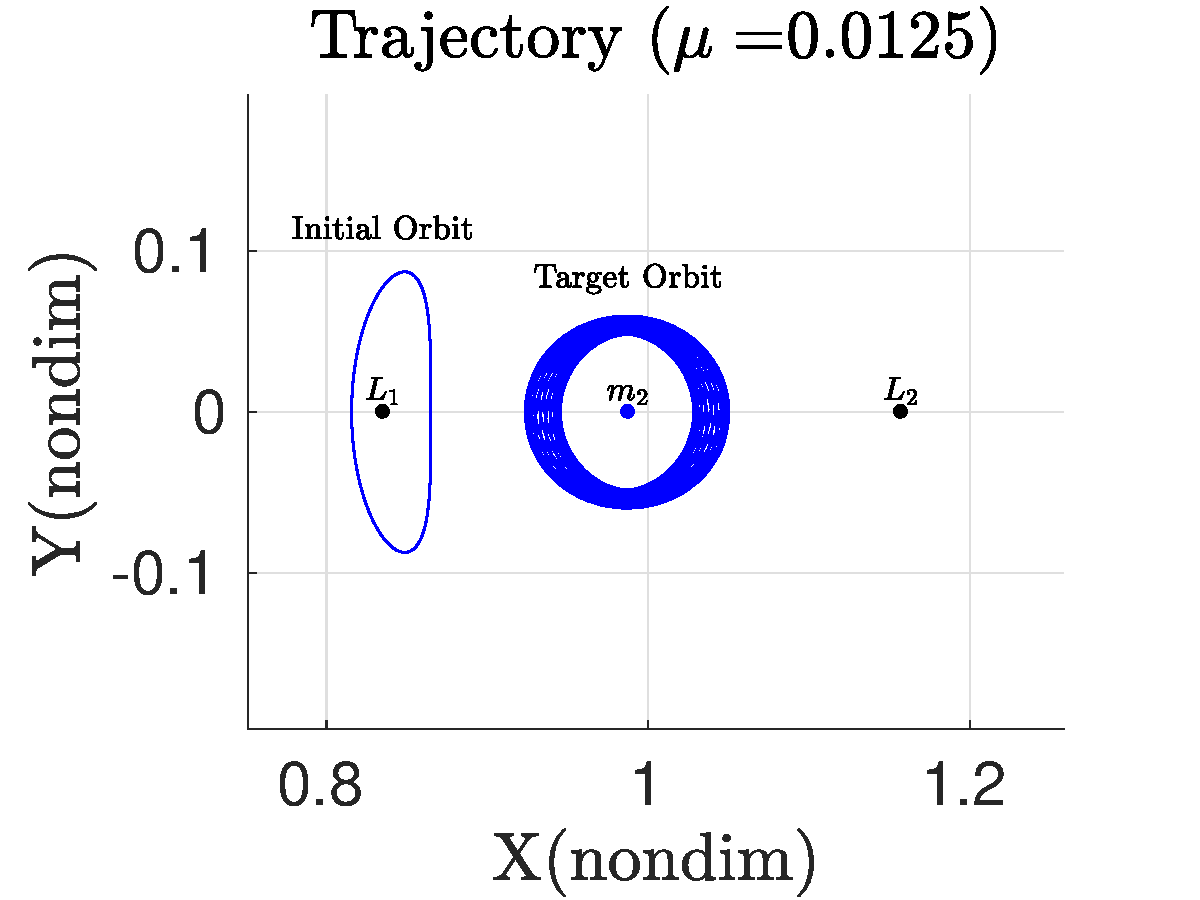
\includegraphics[width=0.5\textwidth]{figures/2017_JAS/moon_orbit.pdf} % requires the graphicx package
   \caption{\(L_1\) periodic orbit transfer to orbit of the Moon: Example scenario demonstrating the initial and target orbit.
   Without the low-thrust propulsion, the spacecraft is constrained to the initial periodic orbit. 
   We determine the reachability set to find a transfer trajectory to the target orbit about the moon.}
   \label{fig:moon_orbit}
\end{figure}
\Cref{fig:moon_orbit} shows that the target set remains in the vicinity of the Moon, or \( m_2\), in the rotating reference frame. 
This type of orbit would be useful for a variety of mission scenarios.
For example, a series of communication satellites could be placed in this type of orbit. 
The bounded trajectories of the vehicles and constant line of sight to both the Moon and the Earth would allow for constant communication for future manned missions and potential habitats.
The initial set is a planar periodic orbit about \( L_1\), which is generated using the process of differential correction of a linear approximation~\cite{koon2011}.

% invariant manifold transfer
As a source for comparison, the method of using invariant manifolds, introduced in~\cite{koon2011}, is implemented.
As described in~\cref{sec:invariant_manifold}, these invariant manifolds are the set of trajectories that either asymptotically arrive or depart the periodic orbit. 
We generate the unstable manifold associated with the initial planar periodic orbit.
We numerically propagate the unstable manifold forward in time until the trajectories intersect the \Poincare section \( y = 0 \).
\Cref{fig:manifold_trajectory} shows the unstable invariant manifold generated from the initial \( L_1\) periodic orbit. 
The blue points in~\cref{fig:manifold_poincare} are the intersections of the target Moon orbit and the \Poincare section.
The two circular regions are the ascending (right) and descending (left) intersections of the target orbit and \Poincare section.
The green points in~\cref{fig:manifold_poincare} are intersections of the unstable manifold from~\cref{fig:manifold_trajectory} with the \Poincare section \( y = 0 \).
Only a single branch of the invariant manifold intersects with the ascending region of the target orbit.
There are no intersections of the invariant manifold with the descending region of the target orbit.
The numerical values associated with the green points denote the required time of flight along the invariant manifold in non-dimensional units.
The required travel time for a transfer using the unstable invariant manifold is  approximately \( t_f \approx 3.1\) non-dimensional time units.
\begin{figure} 
        \centering 
        \begin{subfigure}[htbp]{0.5\textwidth} 
            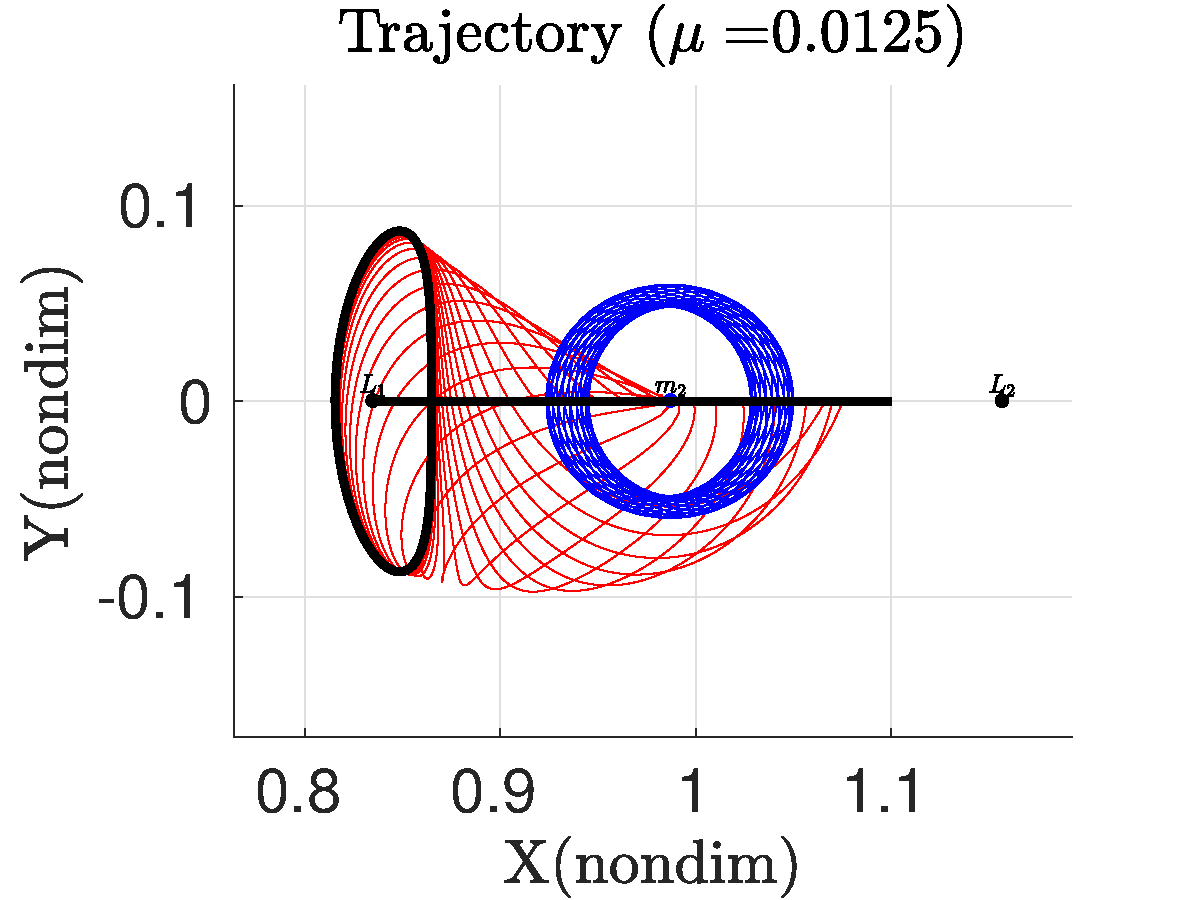
\includegraphics[width=\textwidth]{figures/2017_JAS/manifold_trajectory} 
                \caption{Position space view of invariant manifold} \label{fig:manifold_trajectory} 
        \end{subfigure}~ %
        \begin{subfigure}[htbp]{0.5\textwidth} 
            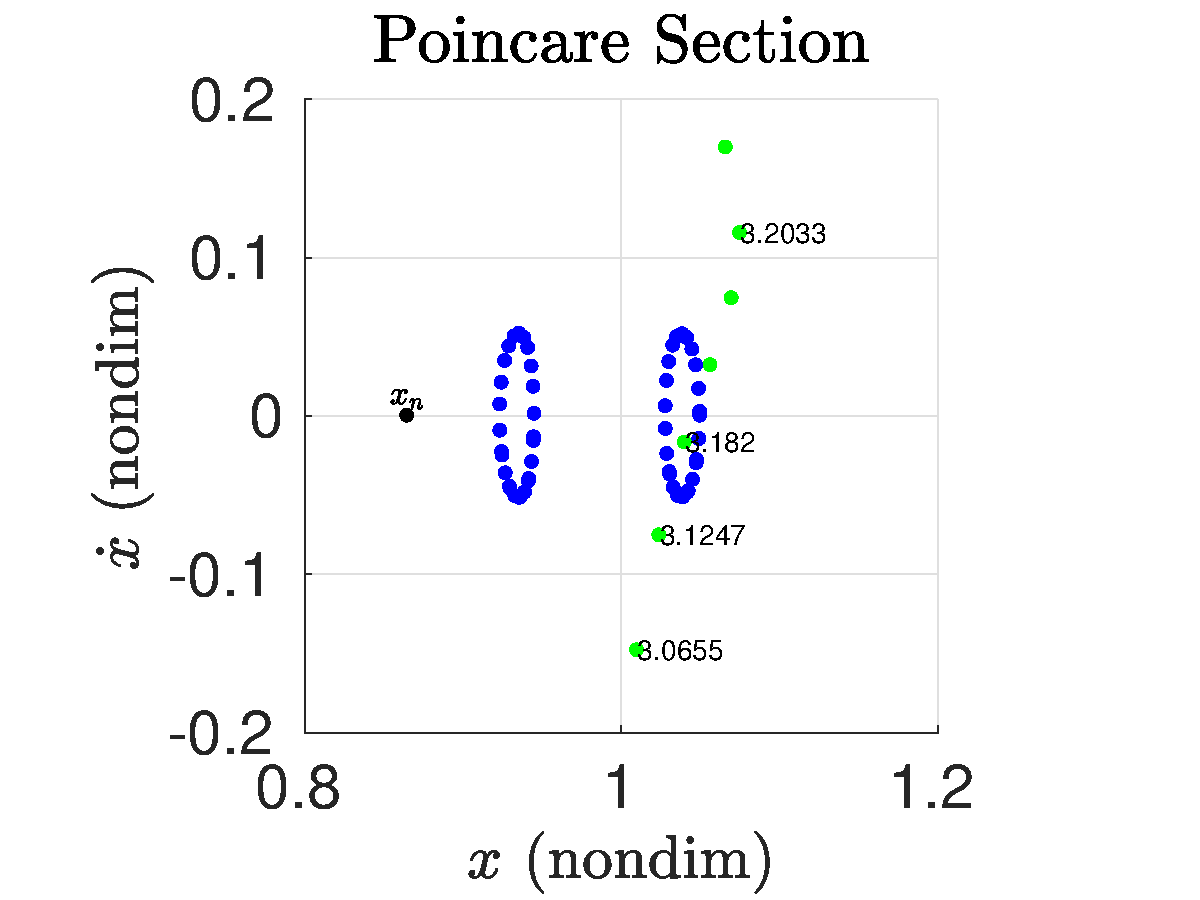
\includegraphics[width=\textwidth]{figures/2017_JAS/manifold_poincare} 
                \caption{\Poincare intersection of invariant manifold (green), target orbit (blue) and the initial orbit (black)} \label{fig:manifold_poincare} 
        \end{subfigure} 
        \caption{Invariant manifold transfer: An example transfer using the invariant manifolds is shown in both the position and \Poincare spaces.
        The control free transfer from the initial periodic orbit to the target orbit result in a long time of flight. 
    In addition, the manifold only intersects the target orbit on the ascending or far side of the moon.}
        \label{fig:invariant_manifold_transfer} 
\end{figure}

Next, we determine the reachability set with addition of a low-thrust control input over a fixed time horizon.
In~\cref{fig:varying_tf_reachability_sets}, we demonstrate the effect of variations in the choice of maximum control bound and terminal time.
While~\cref{sssec:periodic_orbit_transfer} show a specific example of a transfer design process using the intersection of the reachability set on the \Poincare section.
The analysis presented in the following sections define a maximum magnitude of the thrust as \( u_{m} \) and assume that the trust can be directed arbitrarily within the plane. 
This model is representative of many spacecraft which have a body fixed thruster and attitude control system.
Assuming a fully actuated spacecraft model allows us to decouple the translation and rotational dynamics of the spacecraft.

\paragraph{Reachability Set on the \Poincare section}
From the initial state on the periodic orbit, a series of optimal trajectories are generated to determine the reachable set.
The multiple shooting approach is implemented to solve the optimal control problem. 
We divide the time horizon into two equal length segments. 
The state trajectory is initialized using the free trajectory of the periodic orbit. 
Similarly, the costate trajectory is initialized from an initial guess of \( \vc{\lambda}_0 = \begin{bmatrix} -1 & -1 & -1 & -1\end{bmatrix}^T\) and propagated using the system dynamics.
This results in the initial guess of the design vector \( \vc{\chi} = \begin{bmatrix} \vc{\lambda}_0 & \vc{x}_1^{-} & \vc{\lambda}_1^{-} & \vc{\beta} \end{bmatrix}^T\).
This design vector is then varied to ensure that the necessary conditions of optimality and the interior point constraints are satisfied. 
\Cref{tab:varying_tf} shows the range of terminal times, \( t_f \), and maximum control bound, \( u_m \), which are used to investigate their effect on the subsequent reachable set on the \Poincare section.
\begin{table}
    \centering
    \begin{tabular}{ll}  
        \toprule
        \(t_f\) & \( u_m \) \\
        \midrule
        1.24 & 0.05 \\
        1.30 & 0.25 \\
        1.37 & 0.5 \\
        1.44 & \\
        \bottomrule
    \end{tabular}
    \caption{Combinations for \( t_f \) and \( u_m\) used to generate the reachability sets in~\cref{fig:varying_tf_reachability_sets}~\label{tab:varying_tf}}
\end{table}

The angle \( \theta_d\) in~\cref{eq:constraints} is varied to select a different direction along the \Poincare section to maximize.
We discretely vary the angle over the range \( \ang{0} \leq \theta_d < \ang{360} \) to approximate the reachability set of the spacecraft.
Choosing a new angle \( \theta_d \) corresponds to a different direction as well as a new optimal control problem which is again solved using the multiple shooting approach laid out previously.
Each optimal control solution, corresponding to a discrete value of \( \theta_d \), is solved using \texttt{fsolve} as described earlier. 
Each solution on the reachability set is computed in approximately \SI{2}{\minute} on a desktop computer using an \SI{3.4}{\giga\hertz} Intel i7-3700.
The intersection of the optimal trajectories as well as those of the target Moon orbit with the \Poincare section are shown in~\cref{fig:varying_tf_reachability_sets}.

\begin{figure}
    \subcaptionbox{Position space view of reachability sets\label{fig:varying_tf_trajectory}}{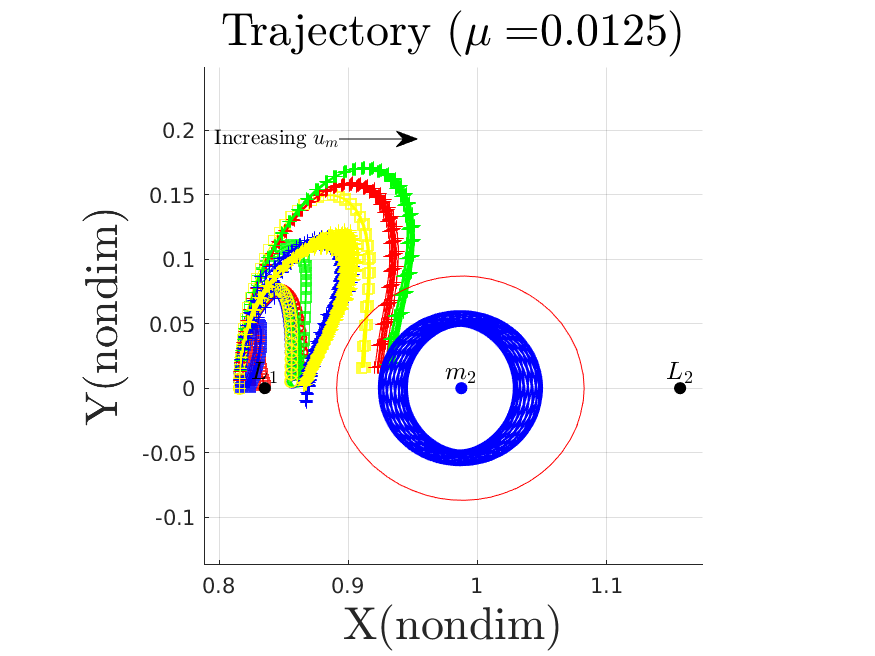
\includegraphics[width=0.5\textwidth]{figures/2017_JAS/trajectory_varying_um.pdf}}~
    \subcaptionbox{\Poincare section view of reachability sets\label{fig:varying_tf_poincare}}{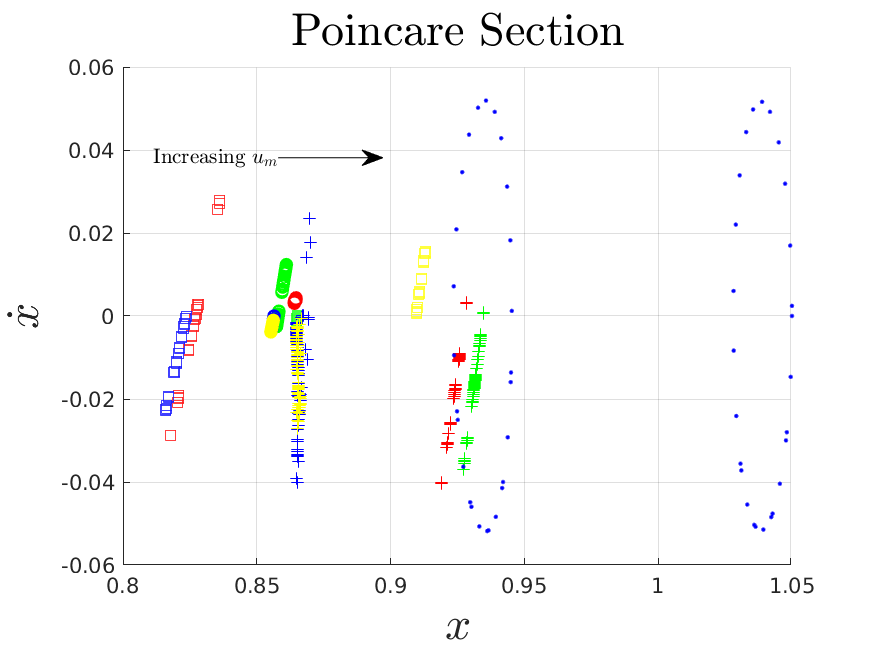
\includegraphics[width=0.5\textwidth]{figures/2017_JAS/poincare_section_varying_um.pdf}}
    \caption{Variation of \( t_f \) and \( u_m\) on the reachability set. 
        Colors, \braces{\text{red}, \text{blue}, \text{green}, \text{yellow}}, are used note increasing \( t_f\) while markers, \braces{\text{circle}, \text{square}, \text{cross}}, are used to denote increasing \(u_m\).
    Increasing the maximum control bound has a large effect and enables the reachability set to intersect the target manifold. 
    Increases in \(t_f\) are less critical and have minimal impact on the distribution of the reachability set on the \Poincare section.~\label{fig:varying_tf_reachability_sets}}
\end{figure}

\Cref{fig:varying_tf_reachability_sets} shows the reachabilty set for twelve combinations of \(t_f\) and \( u_m\) listed in~\cref{tab:varying_tf}.
With a small maximum control bound, \( u_m = \num{0.05} \) shown using square markers, the reachable set is not dramatically changed from that of the no control solution.
The reachable set is denoted using square markers on the left most portion of \cref{fig:varying_tf_poincare}.
Variations of \( t_f\) are indicated using different colors and also demonstrate that this parameters has a smaller impact than changes in \( u_m \).
Increasing the control bound to \( u_m = \num{0.25} \) and \( u_m = \num{0.5} \) shows that the reachable set progressively approaches the target set.

The reachable sets presented in~\cref{fig:varying_tf_reachability_sets} are highly dependent on the initial condition, terminal time, and maximum control bound. 
This example demonstrates that increasing the \( u_m \) results in a larger displacement between the controlled and uncontrolled trajectories.
The reachable set is enlarged from a single point, as shown in~\cref{fig:manifold_poincare} by the black point, to a larger region as shown in~\cref{fig:varying_tf_poincare}.
The choice of \( u_m\), \( t_f \) and initial condition all combine to change the resulting reachability set. 

\paragraph{Transfer to Periodic Orbit}~\label{sssec:periodic_orbit_transfer}
% reachable set transfer
Here we use the results of the preceding section to demonstrate one specific example of a transfer designed using the reachability set.
The acceleration limit is chosen as  \( u_{max} = 0.75 \approx \SI{2}{\milli\meter\per\second\squared} \) in the Earth-Moon system.
Assuming a fixed spacecraft mass of \SI{500}{\kilo\gram}, this model defines a maximum thrust of approximately \SI{1}{\newton}.
Currently, the NASA NEXT xenon thruster is able to provide approximately \SI{0.25}{\newton} of thrust, and a cluster of such engines could be used to provide the desired thrust used in this work~\cite{schmidt2008}.
The trajectories are generated from a fixed initial state of \( \vc{x}_0 = \begin{bmatrix}0.8156 & 0 & 0 & 0.1922 \end{bmatrix}^T \) over a fixed time span of \( t_f = 1.4 \).
This initial state lies on the initial periodic orbit and the time of flight is equivalent to one half period of the initial periodic orbit. 

% discuss reachability set computation
The optimal trajectories, under the influence of the control input \( \vc{u} \), are plotted in red in~\cref{fig:reach_trajectory}.
Initially, the spacecraft is assumed to lie on the periodic orbit.
As a result, the intersection of this periodic orbit with the \Poincare section are two points corresponding to the two crossing of the orbit.
We show the control-free intersection, \( \vc{x}_n \), of the periodic orbit on the \Poincare section in~\cref{fig:manifold_poincare,fig:poincare_compare}
The use of the continuous low thrust propulsion expands the reachable set to region bounded by the red markers in~\cref{fig:poincare_compare}.
The reachable set is an ellipsoidal region with a major axis aligned along \( \theta \approx \ang{70} \) as compared to a fixed point without any control input.
\begin{figure} 
        \centering 
        \begin{subfigure}[htbp]{0.5\textwidth} 
            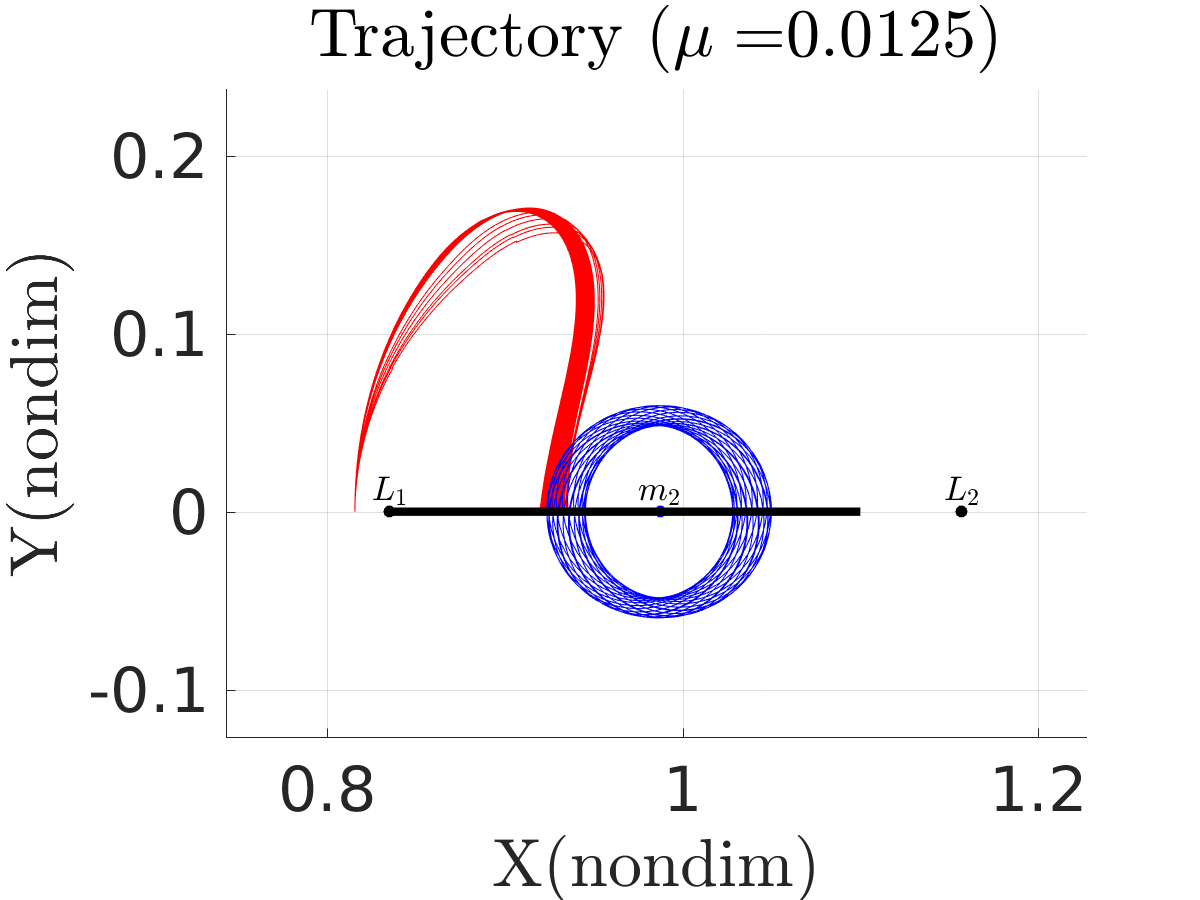
\includegraphics[width=\textwidth]{figures/2017_JAS/reach_trajectory} 
                \caption{Position space view of reachability set} \label{fig:reach_trajectory} 
        \end{subfigure}~ %add desired spacing between images, e. g. ~, \quad, \qquad, \hfill etc. %(or a blank line to force the subfigure onto a new line) 
        \begin{subfigure}[htbp]{0.5\textwidth} 
            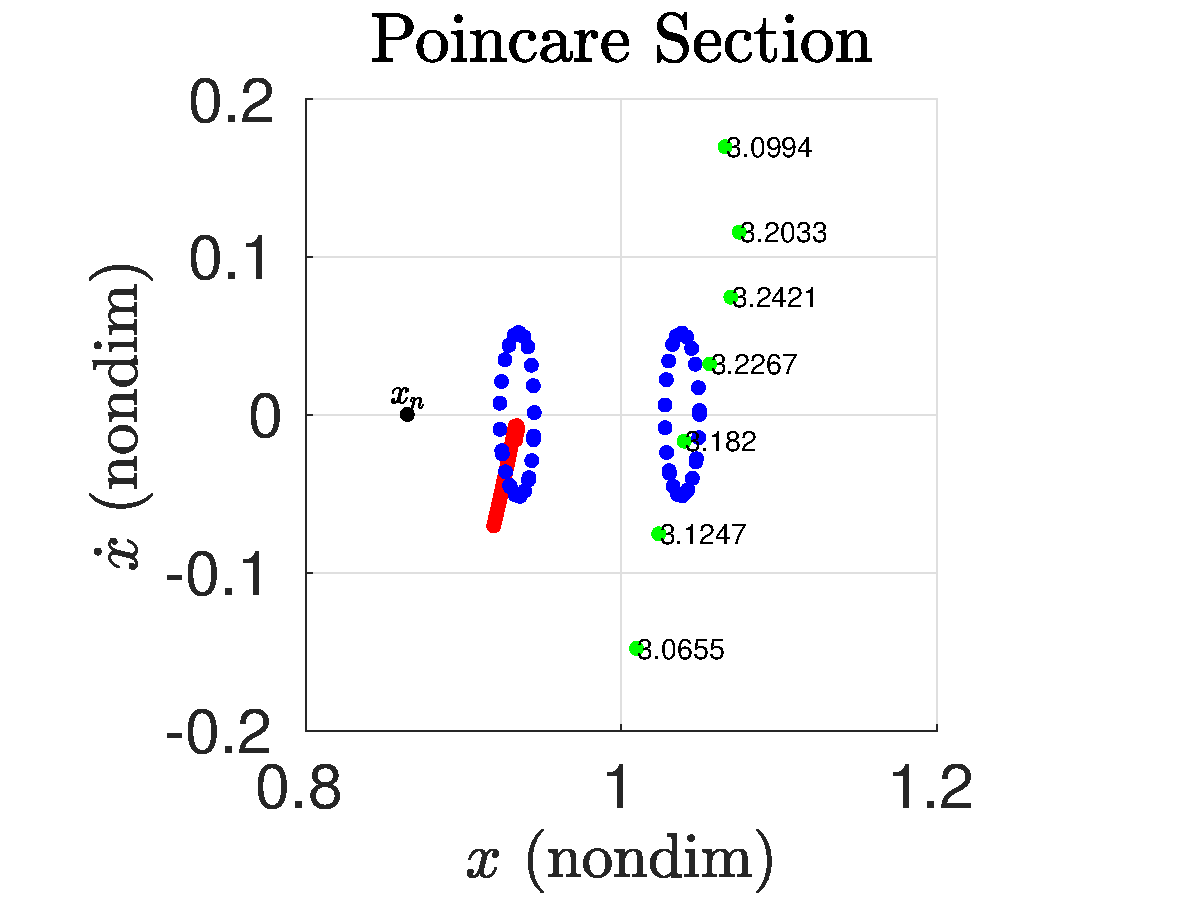
\includegraphics[width=\textwidth]{figures/2017_JAS/poincare_compare} 
                \caption{\Poincare section view of reachability set} \label{fig:poincare_compare} 
        \end{subfigure} %add desired spacing between images, e. g. ~, \quad, \qquad, \hfill etc. %(or a blank line to force the subfigure onto a new line) 
                
        \begin{subfigure}[htbp]{0.5\textwidth} 
            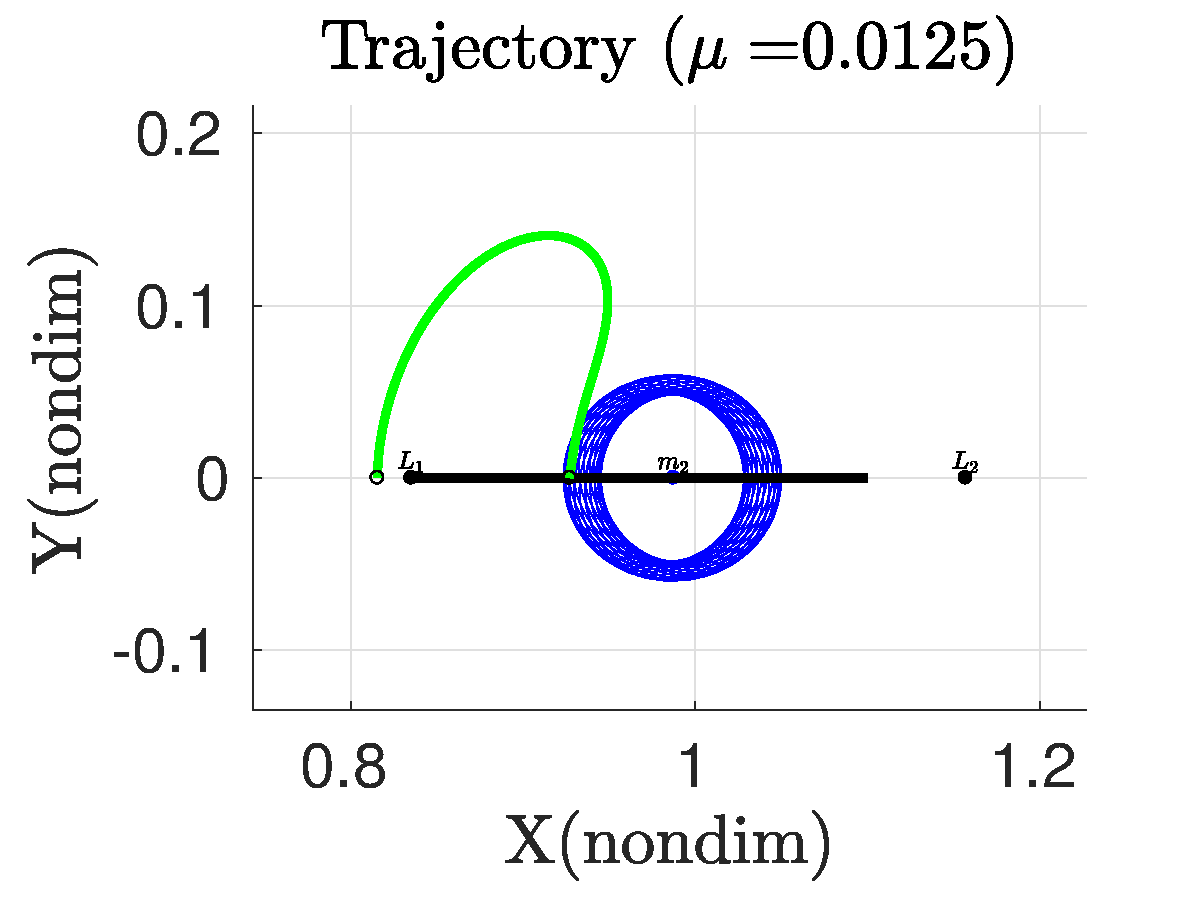
\includegraphics[width=\textwidth]{figures/2017_JAS/reach_transfer} 
                \caption{Transfer trajectory selected from reachability set viewed in the position space} \label{fig:reach_transfer} 
        \end{subfigure}~ 
        \begin{subfigure}[htbp]{0.5\textwidth} 
            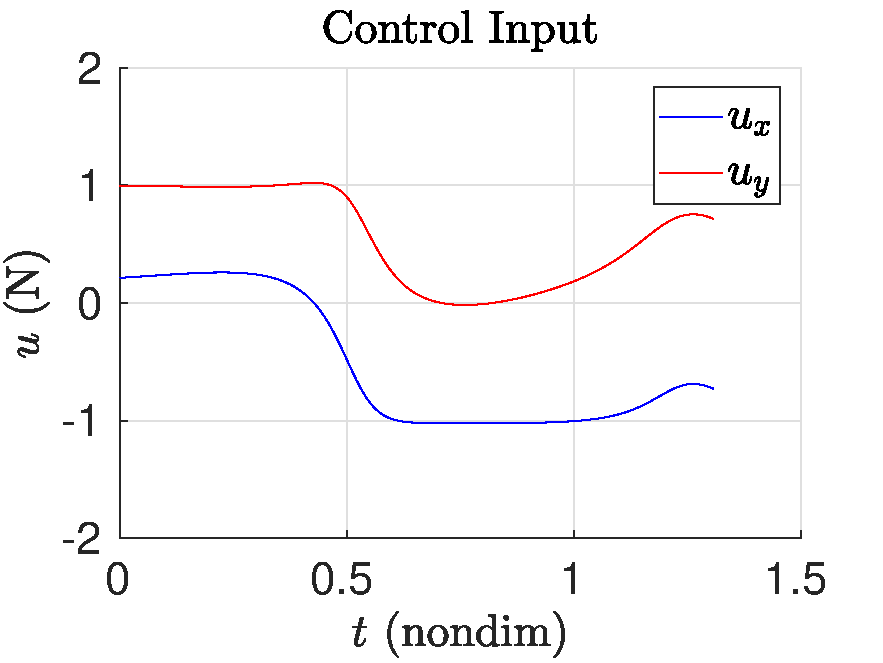
\includegraphics[width=\textwidth]{figures/2017_JAS/control_input_l1} 
                \caption{Control input for the selected transfer trajectory} \label{fig:control_l1} 
        \end{subfigure}~

        \begin{subfigure}[htbp]{0.5\textwidth} 
            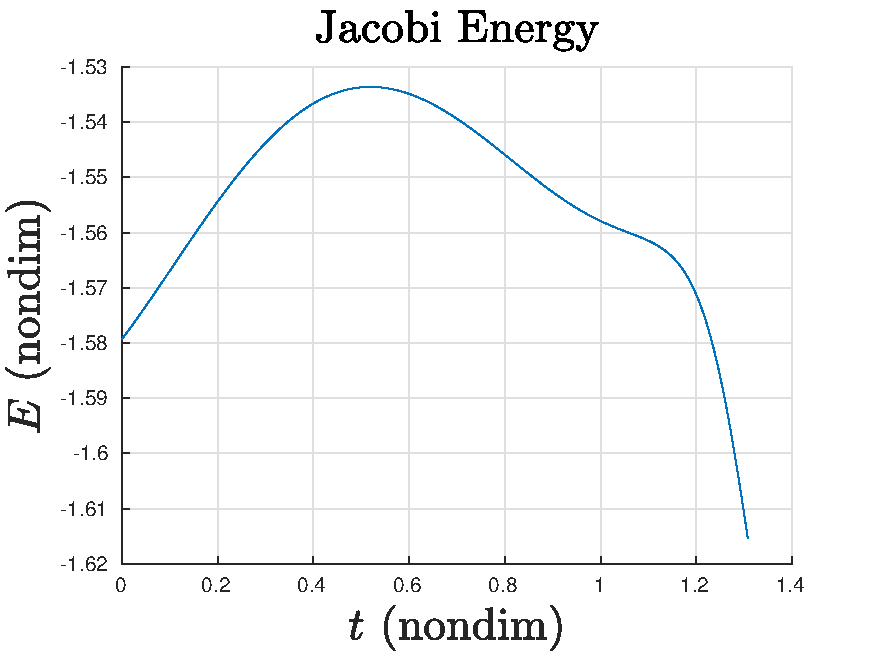
\includegraphics[width=\textwidth, keepaspectratio]{figures/2017_JAS/jacobi.pdf} 
            \caption{Jacobi Energy over transfer \label{fig:jacobi_l1}} 
        \end{subfigure} 

        \caption{\( L_1 \) Reachability set transfer: The low thrust propulsion is used to approximate the reachability set starting from the initial periodic orbit over a fixed time horizon.
            The reachability set is shown in~\cref{fig:reach_trajectory,fig:poincare_compare} in both the position and \Poincare space respectively.
            From this reachability set we chose a trajectory which intersects the target orbit and it is shown in~\cref{fig:reach_transfer}.
        The optimal control to achieve this transfer is shown in~\cref{fig:control_l1}.}
        \label{fig:reachability_set_transfer} 
\end{figure}

% generate the optimal transfer
\Cref{fig:poincare_compare} shows that the reachable set and those of the descending target region intersect.
As both regions are discretely approximated a linear interpolation is used to determine the exact intersection state on the \Poincare section.
This intersection generates a partial target state of \( x_t \text{ and } \dot{x}_t \).
Using the energy level of the target region, defined by~\cref{eq:jacobi}, and the intersection state we can calculate the final component \( \dot{y} \). 
This results in a complete target state \( \vecbf{x}_t \) which lies on the reachable set and on the target orbit. 
A final optimal trajectory is generated such that the \( \vecbf{x}(N) = \vecbf{x}_t \).
This transfer trajectory is denoted by the green path in~\cref{fig:reach_transfer}.
The optimal control input is shown in~\cref{fig:control_l1}. 
The spacecraft achieves the desired target while satisfying the bounded control input.
The Jacobi energy integral, computed using~\cref{eq:jacobi}, is shown in~\cref{fig:jacobi_l1}.
\Cref{fig:jacobi_l1} shows that the vehicle begins with an energy level equal to the periodic orbit and arrives at the target orbit with the appropriate energy.
The first half of the transfer is associated with and increase in energy as the control is used to transition towards the target orbit which is followed by a energy decrease to the target orbit.
This roughly corresponds with the expected optimal solution of a bang-coast-bang type orbital transfer~\cite{kirk2012}.
Convergence statistics associated for this transfer are shown in~\cref{tab:l1_transfer_stats}.
\begin{table}
    \centering
    \begin{tabular}{llr}  
        \toprule
        Metric    & Value \\
        \midrule
        \texttt{fsolve} objective      & \num{6.03e-15}      \\
        \texttt{fsolve} major iterations       & \num{9}      \\
        \texttt{fsolve} first order optimality & \num{1.88e-13} \\
        Optimal cost       & \num{2.09e-31}      \\
        Execution time & \SI{1.49}{\second}       \\
        \bottomrule

    \end{tabular}
    \caption{Convergence statistics for the periodic orbit transfer\label{tab:l1_transfer_stats}}
\end{table}

% compare the invariant manifold method and reachability set
A transfer along the invariant manifold requires on average \( t_f \approx 3.1 \) as compared to \( t_f \approx 1.4 \) for a transfer using low thrust propulsion and the reachable set.
This long time of flight is typical of transfers using invariant manifolds.
The unstable invariant manifold traverses a large region of the phase space and is dependent on the system dynamics. 
In addition, the invariant manifolds asymptotically arrive and depart from the periodic orbit. 
As a result, it may take an arbitrarily long period of time to depart from the vicinity of the periodic orbit.
In addition, only a small portion of the invariant manifold intersects with the target Moon orbit.
In contrast, the low thrust control input we are able to enlarge the reachability set from a single point, \( x_n\) associated with the periodic orbit, to a larger ellipsoidal region shown in red in~\cref{fig:poincare_compare}.
This achieves an intersection with the target orbit with a much lower time of flight as compared to the invariant manifold method.
In addition, by generating the reachability set we are able to compute the required control input to exactly intersect the target orbit.
This avoids having to compute and accomplish a secondary impulsive maneuver to transition from the invariant manifold to the target orbit.

\paragraph{Geostationary Orbit Transfer}
% motivation - may need to compute several reachability sets
There are many situations where a more complicated and extensive orbital transfer is desired. 
In this section, we present a simulation of transferring from a geostationary orbit to a periodic orbit about the \( L_1 \) Lagrange point.
From this location, it is possible to transition to the Moon, as shown in~\cref{sec:periodic_orbit_transfer}, or beyond the Earth-Moon system through the use of invariant manifolds~\cite{koon2011}.
This type of low energy transfer would be most suitable for unmanned spacecraft transitioning from the Earth to the Moon.
The long time of flight would make such a transfer unsuitable for manned missions due to life support constraints.
Future proposals for permanent lunar spacecraft and bases will require frequent supply missions to remain viable. 
Transfers from the Earth to the Lagrange points, through the use of low-thrust electric propulsion, offer an additional and potentially shorter time of flight in comparison to the low-energy transfers which utilize solar perturbations.

\Cref{sec:periodic_orbit_transfer} demonstrated the capability of determining an orbital transfer after locating the intersection of the reachability set and a target orbit.
However, it may not be possible to achieve an intersection on the \Poincare section after a single iteration. 
Since the spacecraft has an upper bounded control input and time of flight the reachability set is finite in size. 
As a result, we present a method of performing several iterations of the reachability set computation. 
A straightforward method is presented which allows for a series of reachability sets to be computed which progressively move the trajectory towards the target.
In this manner, it is possible to determine more complicated transfers by a simple selection of states from the reachability set.
This affords a systematic method of determining general transfer trajectories in the three body problem.

% discuss difficulties in applying direct optimization or the invariant manifold method
It is possible to design arbitrary transfers using either a direct optimization or invariant manifold based approach.
The direct optimization method transforms the optimal control problem into a nonlinear programming problem.
Instead of solving the Euler-Lagrange equations the state and control histories are parameterized and solved through any number of mathematical programming methods.
However, due to this parameterization only an approximate solution, which approximates the true optimal solution in the limit, is feasible. 
On the other hand, our method applies an indirect optimization method.
The necessary conditions for optimality are computed and directly solved in generating the reachability set. 
The use of the reachability set also avoids the issues of selecting a valid initial condition.
We select a state on the maximum reachability set which minimizes the distance toward the target. 
This straightforward approach achieves an optimal trajectory and is used to generate general transfers.

The invariant manifold method is difficult to apply to general orbital transfers. 
The manifolds are associated with periodic orbits in the three-body system. 
In this case, an appropriate periodic orbit must first be determined prior to generating the invariant manifold.
Furthermore, there is no guarantee that the invariant manifold will pass through a desired region of space. 
For example, in the Earth-Moon system the unstable manifolds of periodic orbits about \( L_1 \) do not pass close to the Earth, but rather are beyond the geostationary orbit altitude. 
In addition, determining the intersections between various invariant manifolds is not trivial. 
It requires an appropriate \Poincare~section and the generation of several invariant manifolds.
There is no clear method of selecting the periodic orbits required based on the type of transfer desired. 
Determining an intersection between these invariant manifolds generally requires extended flight times, involving several orbits of the primaries, before an appropriate intersection is found.
As a result, it is difficult to generalize this method to arbitrary transfers in the three-body problem.

% describe initial and target states for this example
This numerical simulation demonstrates the ability of the our approach to determine more general transfer trajectories in the \gls{pcrtbp}. 
We use multiple iterations of the reachability set to achieve a more complicated transfer.
In this manner, it is possible to design arbitrary transfers which are not possible using a single reachability computation.
Initially, it is assumed that the spacecraft lies on a circular geostationary orbit in the non-dimensional Earth-Moon three-body system. 
While the geostationary orbit is not a typical ``parking orbit'' for most spacecraft missions it serves as a convenient altitude to demonstrate our approach.
The geostationary orbit about the Earth is transformed into the rotating reference frame of the Earth-Moon three body problem.
In addition, we non-dimensionalize the initial state to find \( \vc{x}_0 = \begin{bmatrix} 0.0972 & 0 & 0 & 3.0010\end{bmatrix}^T\) as the initial condition of the spacecraft on the geostationary orbit.
It is desired to transfer to a periodic orbit about the \( L_1 \) Lagrange point. 
The periodic orbit is defined by the initial condition \(\begin{bmatrix} 0.8057 & 0 & 0 & 0.2982 \end{bmatrix}^T \).
The initial and target orbits are illustrated in~\cref{fig:geo_transfer_target}.
\begin{figure}[htbp]
   \centering
   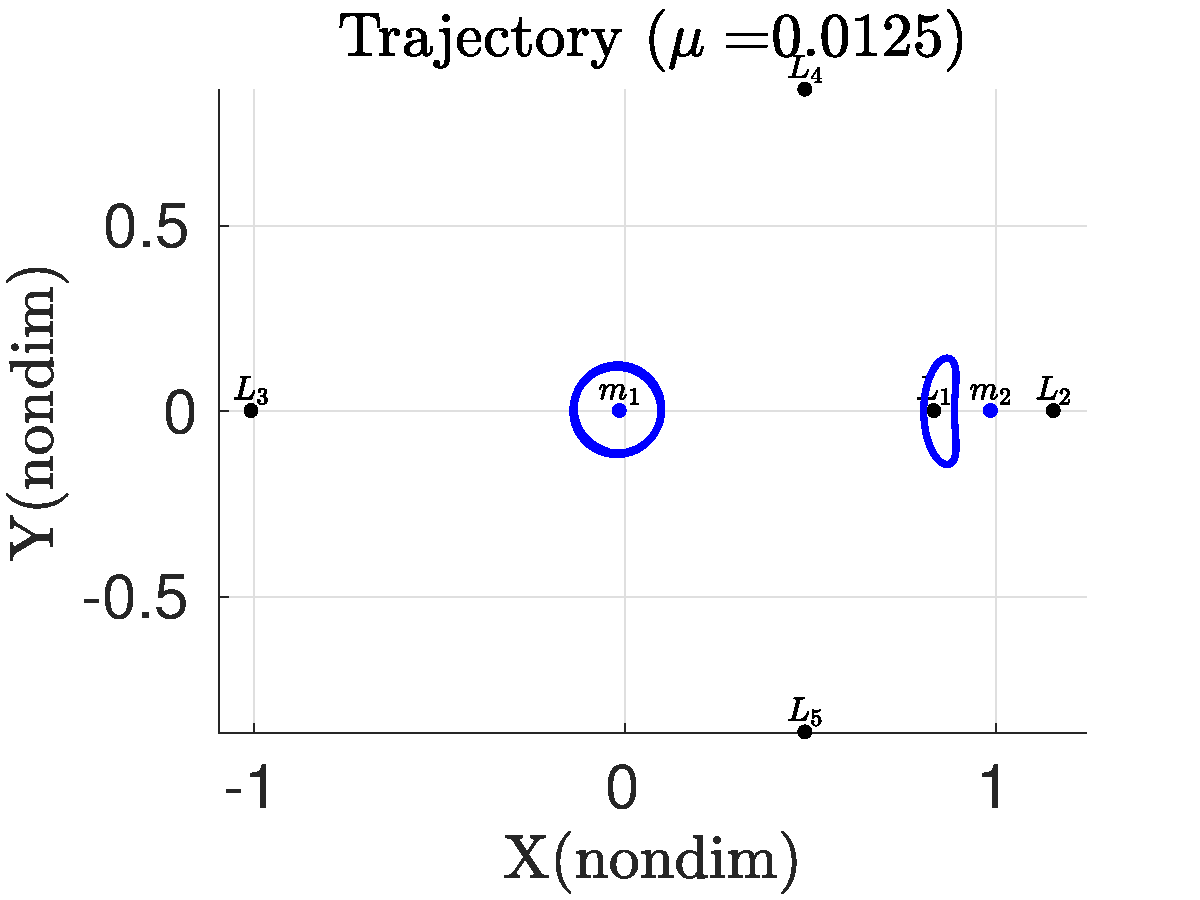
\includegraphics[width=0.5\textwidth]{figures/2017_JAS/initial_final} % requires the graphicx package
   \caption{Geostationary to \( L_1 \) transfer: Representation of the initial and target orbits for the reachability transfer. 
   Vehicle is assumed to begin on the geostationary orbit about \( m_1\) and will transfer to the periodic orbit about \( L_1\)}
   \label{fig:geo_transfer_target}
\end{figure}
In~\cref{fig:geo_transfer_target}, the initial orbit is located in the center of the figure and centered about \( m_1 \) while the target periodic orbit is determined about the \( L_1 \) Lagrange point.
Instead of determining a transfer directly between the geostationary orbit and the periodic orbit, we seek to instead transfer to the stable manifold of the periodic orbit.
This stable manifold will then asymptotically approach the target orbit without any further control input.
Once on the manifold, the spacecraft will coast in an uncontrolled fashion and asymptotically arrive at the desired periodic orbit.

We first generate the stable invariant manifold associated with the periodic orbit in order to determine our target set.
The stable manifold is propagated to the \Poincare section at \( y = 0 \), which is denoted by the horizontal black line in the position space visualizations given in~\cref{fig:stage1to4_reachability,fig:stage5to8_reachability,fig:geo_transfer_full}.
The stable manifold is denoted by the green trajectories which span the majority of the phase space. 
In addition, we plot the intersection of the stable manifold with the \Poincare section with green markers.
The initial orbit and the stable invariant manifold do not intersect and the transfer objective is to enlarge the reachability set to include the stable manifold.

Next, we compute the reachable sets originating on the geo-stationary orbit and subject to the maximum control constraint. 
The multiple shooting approach is used to solve the optimal control problem with two segments.
For the first reachability set computation, the initial geostationary orbit is used to initialize the multiple shooting algorithm.
We use the same initial guess of \( \vc{\lambda}_0\) as in~\cref{sec:periodic_orbit_transfer} and propagate over the fixed time horizon of the period of the geostationary orbit to initialize \( \vc{\lambda}_i^{-}\).

\begin{figure}[htbp]
    \centering
    \begin{subfigure}[htbp]{0.5\textwidth} 
        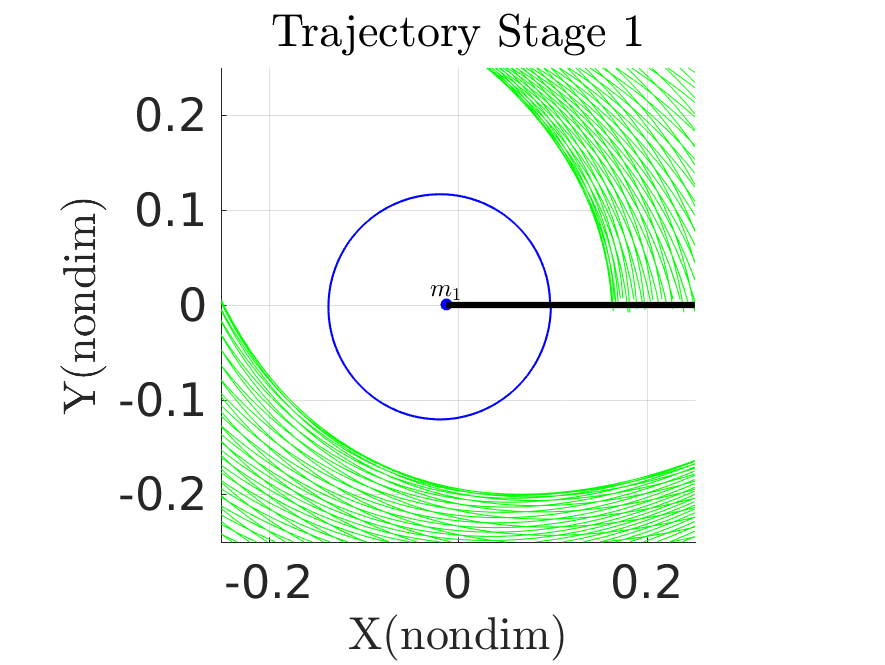
\includegraphics[width=\textwidth, keepaspectratio]{figures/2017_JAS/stage1_trajectory_zoom.pdf} 
        \caption{Stage 1 Trajectory~\label{fig:stage1_trajecotry_zoom}} 
    \end{subfigure}~
    \begin{subfigure}[htbp]{0.5\textwidth} 
        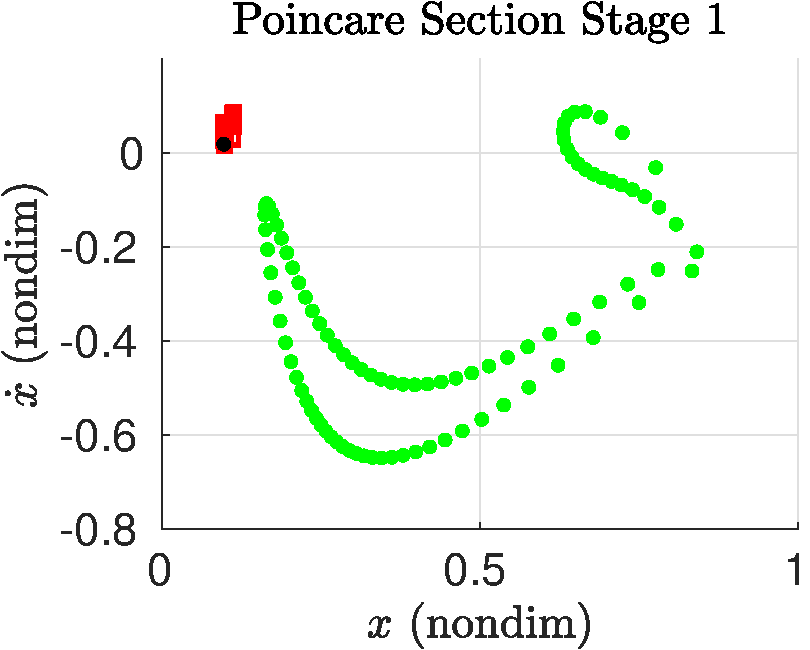
\includegraphics[width=\textwidth, keepaspectratio]{figures/2017_JAS/stage1_poincare.pdf} 
        \caption{Stage 1 \Poincare~section \label{fig:stage1_poincare}} 
    \end{subfigure}


    \begin{subfigure}[htbp]{0.5\textwidth} 
        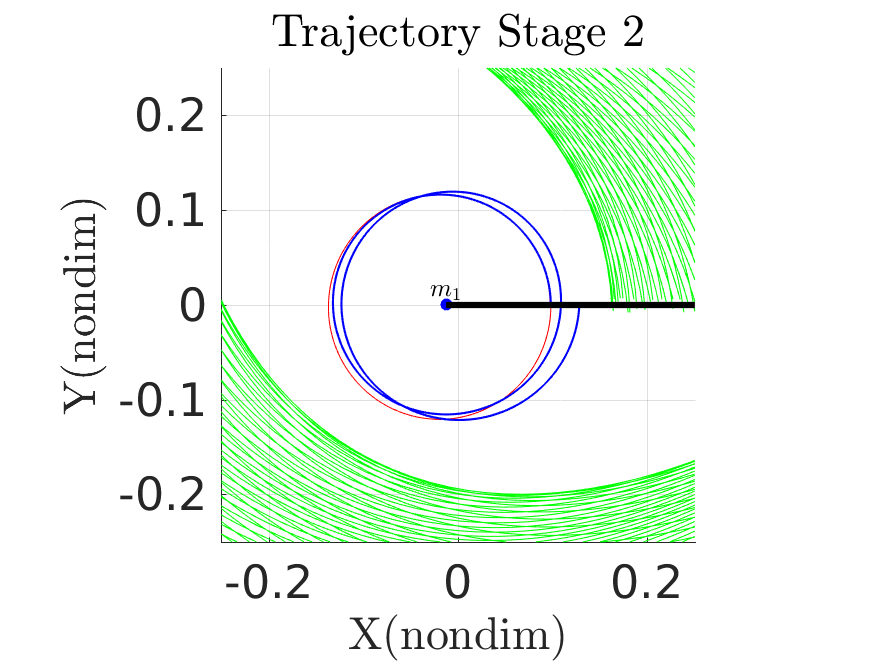
\includegraphics[width=\textwidth, keepaspectratio]{figures/2017_JAS/stage2_trajectory_zoom.pdf} 
        \caption{Stage 2 Trajectory~\label{fig:stage2_trajecotry_zoom}} 
    \end{subfigure}~
    \begin{subfigure}[htbp]{0.5\textwidth} 
        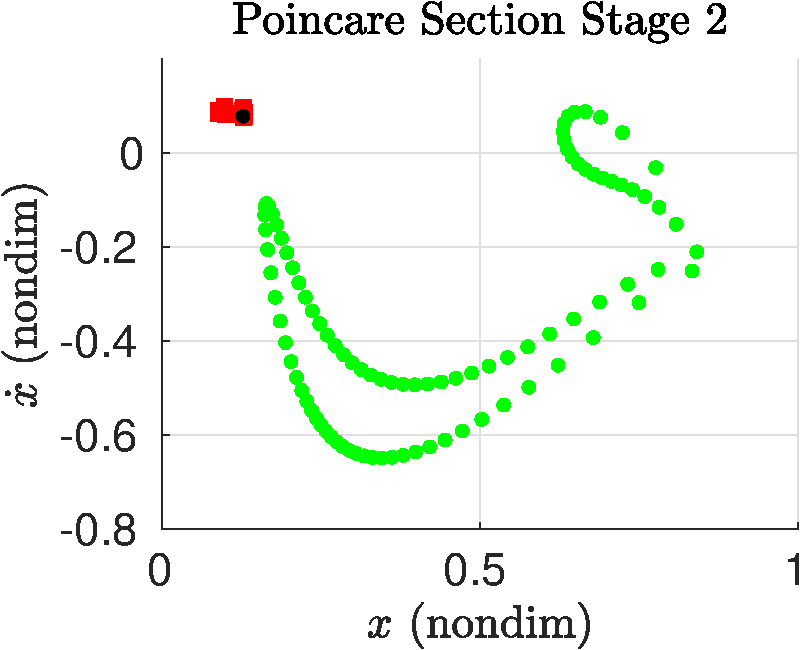
\includegraphics[width=\textwidth, keepaspectratio]{figures/2017_JAS/stage2_poincare.pdf} 
        \caption{Stage 2 \Poincare~section \label{fig:stage2_poincare}} 
    \end{subfigure}

    \begin{subfigure}[htbp]{0.5\textwidth} 
        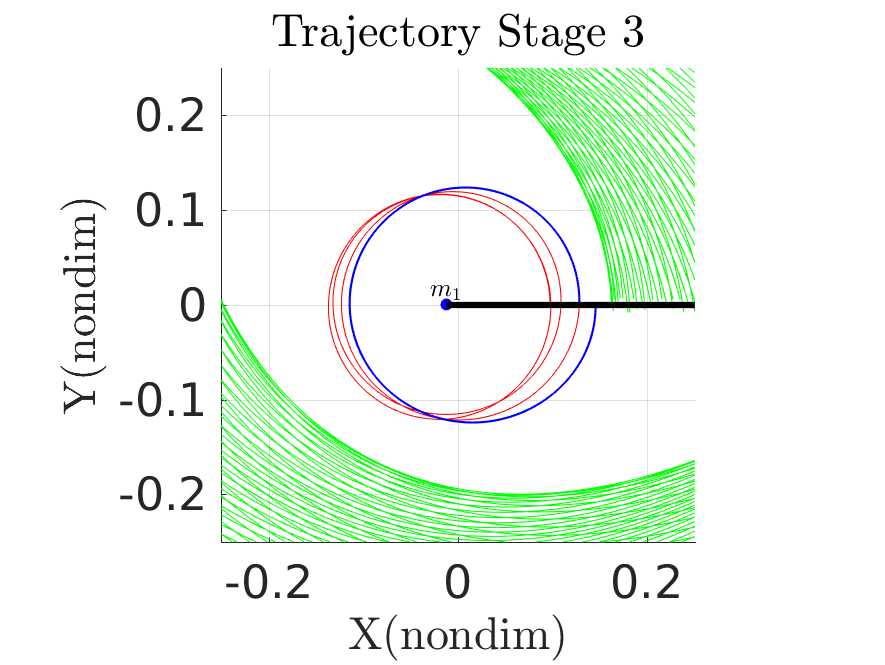
\includegraphics[width=\textwidth, keepaspectratio]{figures/2017_JAS/stage3_trajectory_zoom.pdf} 
        \caption{Stage 3 Trajectory~\label{fig:stage3_trajecotry_zoom}} 
    \end{subfigure}~
    \begin{subfigure}[htbp]{0.5\textwidth} 
        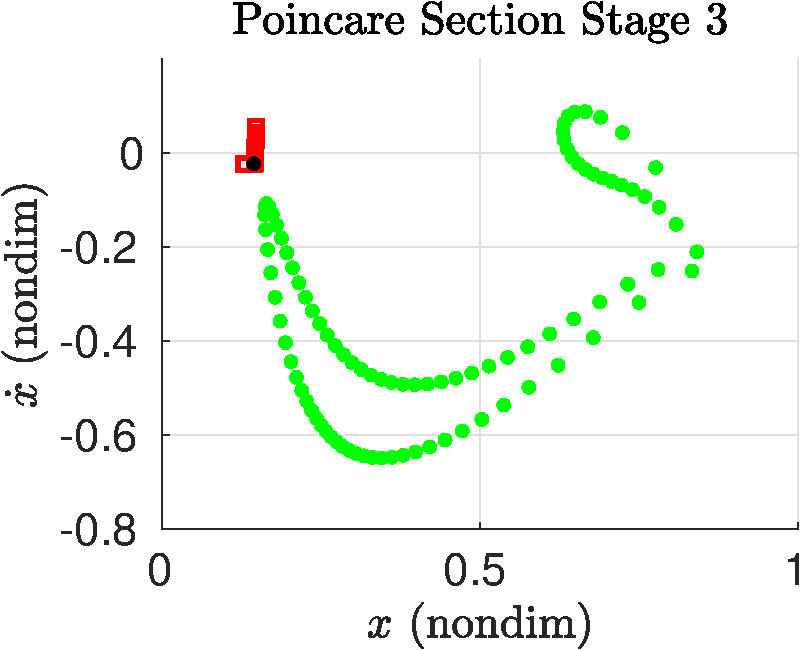
\includegraphics[width=\textwidth, keepaspectratio]{figures/2017_JAS/stage3_poincare.pdf} 
        \caption{Stage 3 \Poincare~section \label{fig:stage3_poincare}} 
    \end{subfigure}
 
    \begin{subfigure}[htbp]{0.5\textwidth} 
        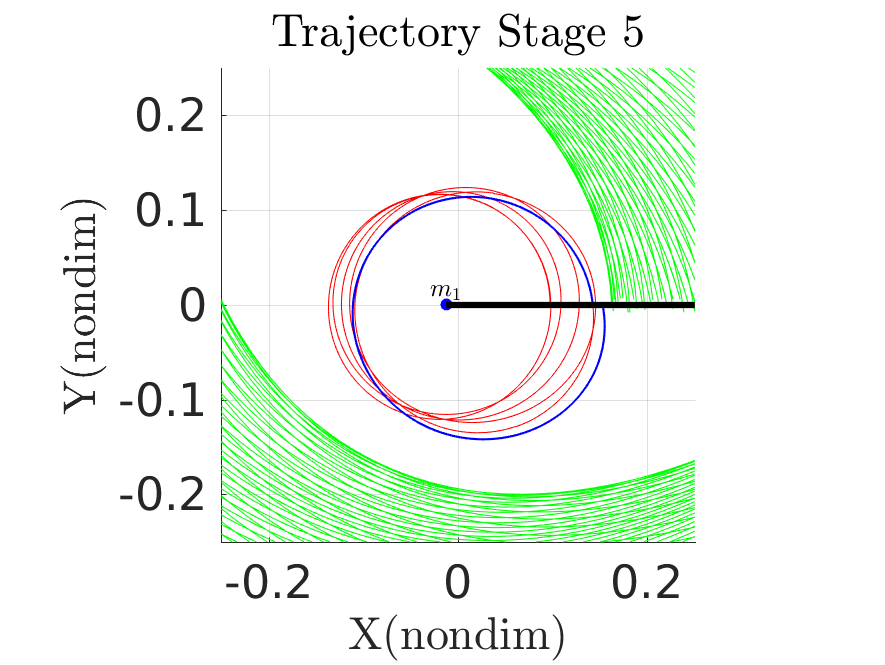
\includegraphics[width=\textwidth, keepaspectratio]{figures/2017_JAS/stage5_trajectory_zoom.pdf} 
        \caption{Stage 4 Trajectory~\label{fig:stage4_trajecotry_zoom}} 
    \end{subfigure}~
    \begin{subfigure}[htbp]{0.5\textwidth} 
        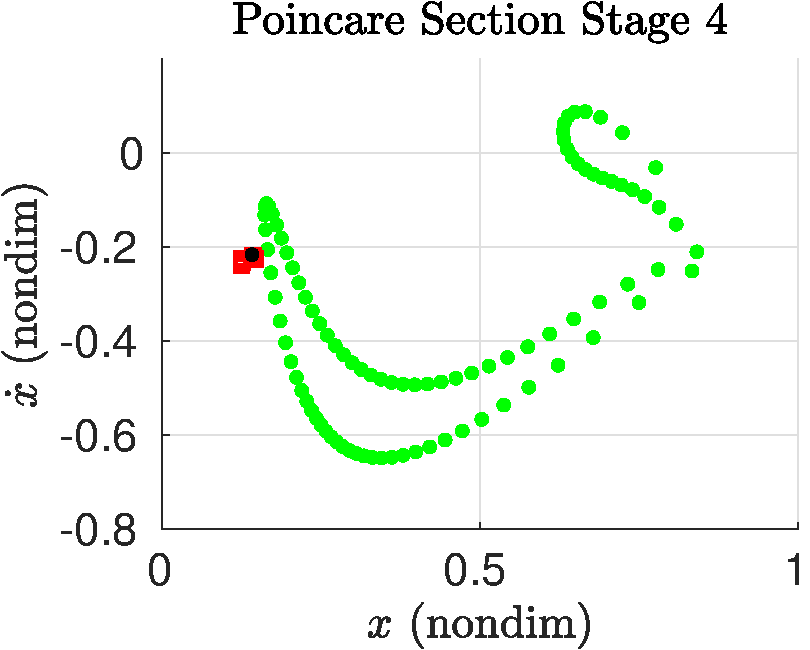
\includegraphics[width=\textwidth, keepaspectratio]{figures/2017_JAS/stage4_poincare.pdf} 
        \caption{Stage 4 \Poincare~section \label{fig:stage4_poincare}} 
    \end{subfigure}   
    \caption{Stage 1-4 reachability sets: The first four reachability sets visualized in both the position (left) and \Poincare space (right).
        The minimum trajectories from the preceding stages are shown in red, while the next stage is shown in blue.
    The transfer goal is to generate a complete trajectory from the initial geostationary orbit to the \( L_1 \) stable manifold, with an eventual arrival at the \( L_1 \) periodic orbit~\label{fig:stage1to4_reachability}}
\end{figure}
The first reachable set is computed beginning on the geostationary orbit at it's intersection with the \Poincare section and we again assume a upper bound on the thrust magnitude of \( u_{max} = 0.75 \).
The reachable set is generated by varying the angle \( \ang{0} \leq \theta < \ang{360} \) in~\cref{eq:constraints} defined on the \Poincare section.
This allows us to approximate the set of states that are achievable in the \( \parenth{x ,\dot{x}} \) space.
The intersection of the first reachable set with the \Poincare section is shown in~\cref{fig:stage1_poincare} in red.
While the reachable set does not intersect the stable manifold, it does reduce some of the distance in the \(\dot{x}\) dimension.
From this reachable set, we chose a trajectory which minimizes the distance towards the stable manifold, which is shown in~\cref{fig:stage1_poincare} by the black marker.
The distance on the \Poincare section between the reachable set and the stable manifolds is defined as the function \( d \),
\begin{align*}
        d(\vc{x}(N)) = \sqrt{\parenth{x - x_t}^2 + \parenth{\dot{x} - \dot{x}_t}^2}.
\end{align*}
From the reachable set, the trajectory which minimizes \( d \) is used to initialize the next iteration.
The minimum trajectory is also shown in~\cref{fig:stage1_trajecotry_zoom} and is used to initialize the following stage.
Over the relatively short time horizon of the geostationary orbital period, the reachability set remains quite close to the initial orbit. 
However, the addition of the control input has increased the velocity component of the trajectory.
It is this velocity change that is subsequently exploited to generate the transfer trajectory.

The minimum trajectory from the first iteration of the reachability set is used to initialize the following stage.
From the terminal state of the first iteration, the second reachability set is computed and displayed in~\cref{fig:stage2_trajecotry_zoom,fig:stage2_poincare}.
The second reachability set is shown on the \Poincare section in~\cref{fig:stage2_poincare}.
This iteration greatly decreases the distance in the \( x \) component between the trajectory and the target, at the expense of a small deviation in the \( \dot{x} \) component.
In~\cref{fig:stage2_trajecotry_zoom}, the first stage trajectory is shown in red while the additional stage is shown in blue, which demonstrates the decrease in the \( x \) component.

\begin{figure}[htbp]
    \centering
    \begin{subfigure}[htbp]{0.5\textwidth} 
        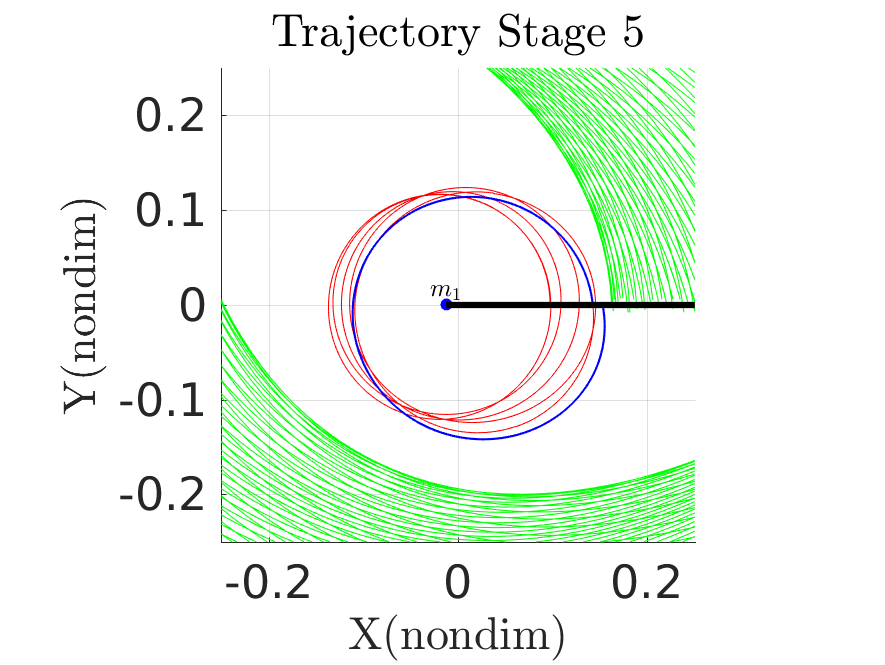
\includegraphics[width=\textwidth, keepaspectratio]{figures/2017_JAS/stage5_trajectory_zoom.pdf} 
        \caption{Stage 5 Trajectory~\label{fig:stage5_trajecotry_zoom}} 
    \end{subfigure}~
    \begin{subfigure}[htbp]{0.5\textwidth} 
        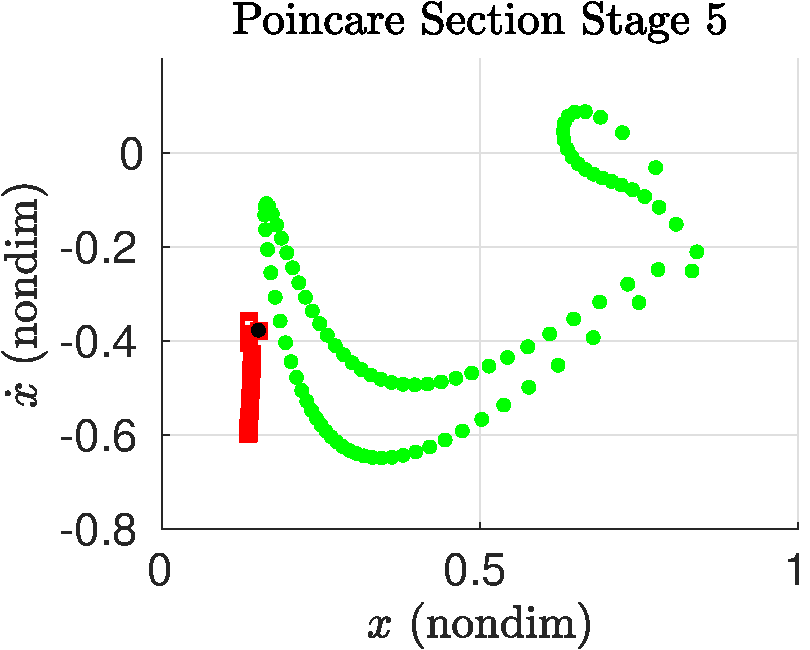
\includegraphics[width=\textwidth, keepaspectratio]{figures/2017_JAS/stage5_poincare.pdf} 
        \caption{Stage 5 \Poincare~section \label{fig:stage5_poincare}} 
    \end{subfigure}

    \begin{subfigure}[htbp]{0.5\textwidth} 
        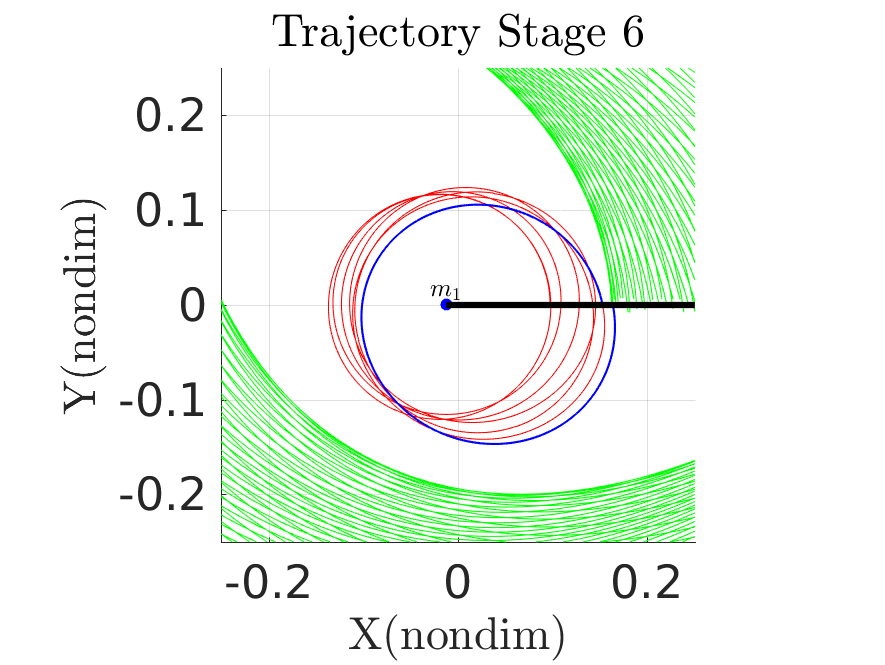
\includegraphics[width=\textwidth, keepaspectratio]{figures/2017_JAS/stage6_trajectory_zoom.pdf} 
        \caption{Stage 6 Trajectory~\label{fig:stage6_trajecotry_zoom}} 
    \end{subfigure}~
    \begin{subfigure}[htbp]{0.5\textwidth} 
        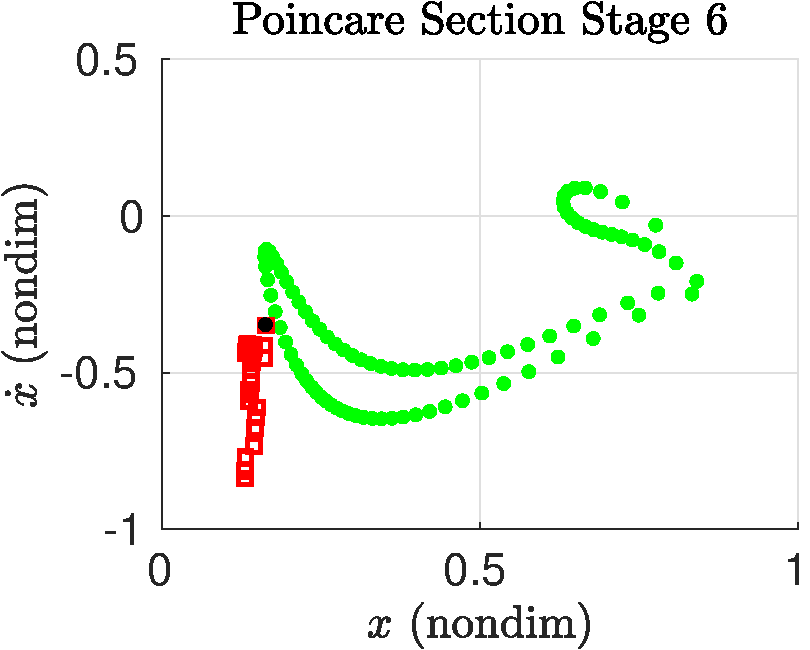
\includegraphics[width=\textwidth, keepaspectratio]{figures/2017_JAS/stage6_poincare.pdf} 
        \caption{Stage 6 \Poincare~section \label{fig:stage6_poincare}} 
    \end{subfigure}

    \begin{subfigure}[htbp]{0.5\textwidth} 
        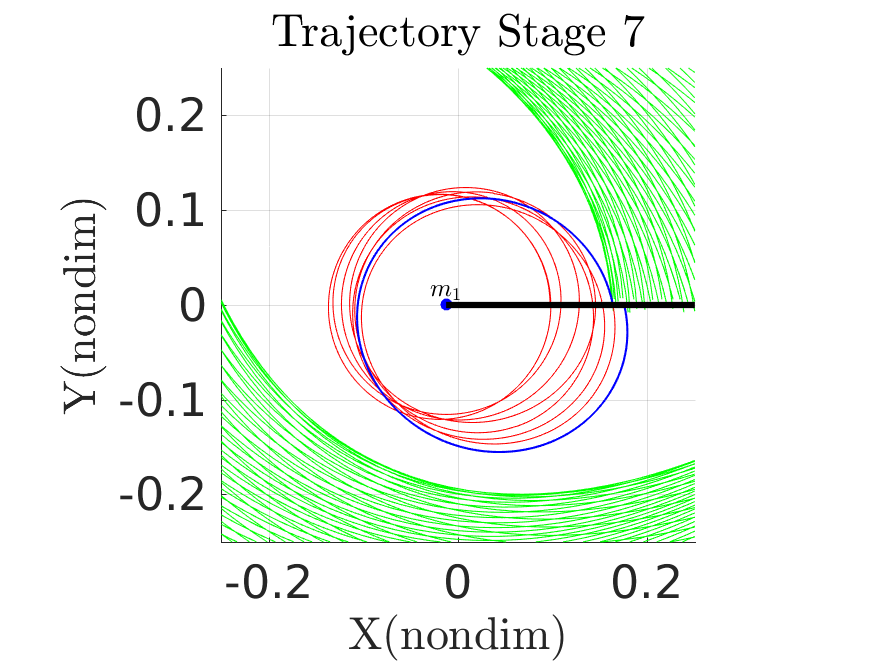
\includegraphics[width=\textwidth, keepaspectratio]{figures/2017_JAS/stage7_trajectory_zoom.pdf} 
        \caption{Stage 7 Trajectory~\label{fig:stage7_trajecotry_zoom}} 
    \end{subfigure}~
    \begin{subfigure}[htbp]{0.5\textwidth} 
        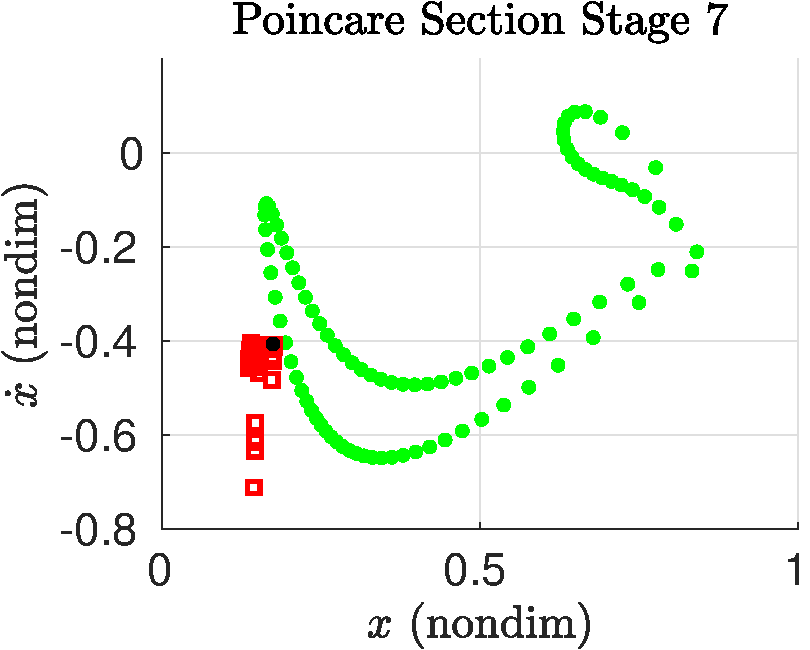
\includegraphics[width=\textwidth, keepaspectratio]{figures/2017_JAS/stage7_poincare.pdf} 
        \caption{Stage 7 \Poincare~section \label{fig:stage7_poincare}} 
    \end{subfigure}
 
    \begin{subfigure}[htbp]{0.5\textwidth} 
        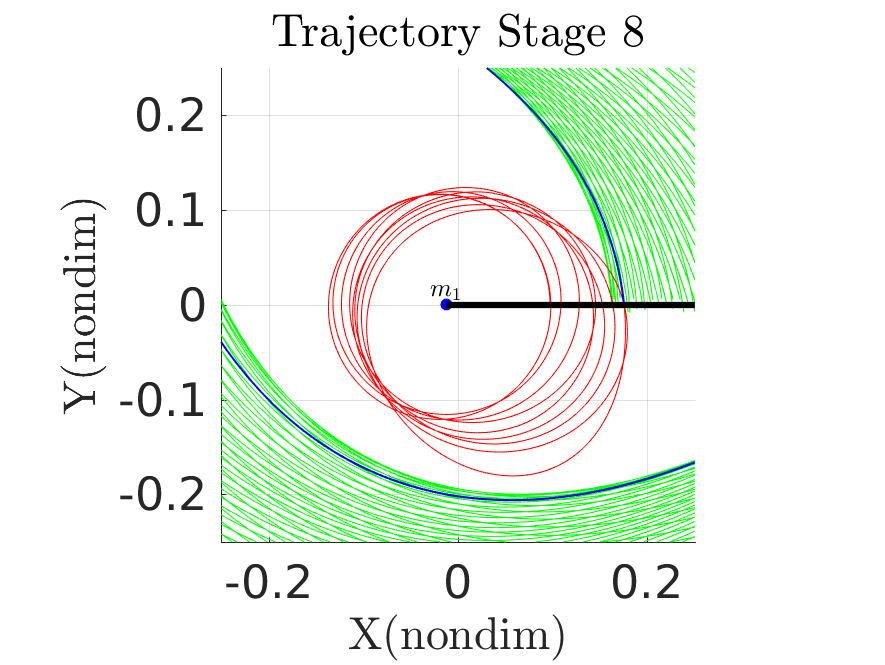
\includegraphics[width=\textwidth, keepaspectratio]{figures/2017_JAS/stage8_trajectory_zoom.pdf} 
        \caption{Stage 8 Trajectory~\label{fig:stage8_trajecotry_zoom}} 
    \end{subfigure}~
    \begin{subfigure}[htbp]{0.5\textwidth} 
        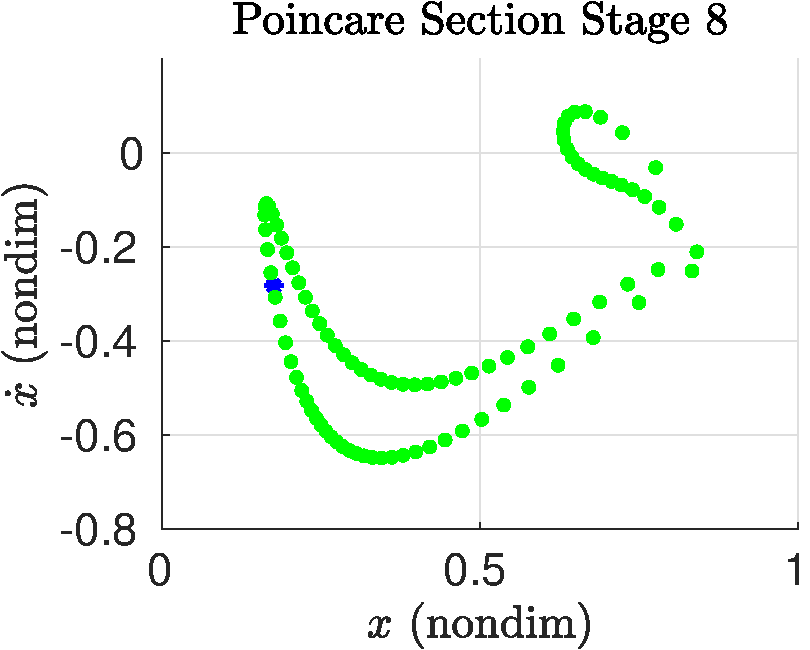
\includegraphics[width=\textwidth, keepaspectratio]{figures/2017_JAS/stage8_poincare.pdf} 
        \caption{Stage 8 \Poincare~section \label{fig:stage8_poincare}} 
    \end{subfigure}   
    \caption{Stage 5-8 reachability sets: The last four reachability sets visualized in both the position (left) and \Poincare space (right).
        The minimum trajectories from the preceding stages are shown in red, while the next stage is shown in blue.
    The transfer goal is to generate a complete trajectory from the initial geostationary orbit to the \( L_1 \) stable manifold, with an eventual arrival at the \( L_1 \) periodic orbit~\label{fig:stage5to8_reachability}}
\end{figure}

With each reachable set we move the controlled trajectory closer to the target stable manifold.
\Cref{fig:stage1to4_reachability,fig:stage5to8_reachability} shows all of the intermediate reachability iterations to transfer between the initial orbit and the stable invariant manifold.
The final reachable set intersects the stable manifold of the periodic orbit. 
A final fixed terminal time and terminal state optimal transfer is finally used to arrive at the stable manifold.
The optimization statistics for the final transfer are shown in~\cref{tab:geo_transfer}.
\begin{table}[h]
    \centering
    \begin{tabular}{llr}  
        \toprule
        Metric    & Value \\
        \midrule
        \texttt{fsolve} objective      & \num{1.42e-11}      \\
        \texttt{fsolve} major iterations       & \num{18}      \\
        \texttt{fsolve} first order optimality & \num{7.2e-11} \\
        Optimal cost       & \num{4.30e-25}      \\
        Execution time & \SI{2.62}{\second}       \\
        \bottomrule
    \end{tabular}
    \caption{Convergence statistics for the geostationary orbit transfer\label{tab:geo_transfer}}
\end{table}
The complete transfer trajectory, after eight iterations, is shown in~\Cref{fig:geo_transfer}. 
Combining these trajectories results in the powered portion of the transfer from the geostationary orbit to the stable manifold. 
Each iteration systematically moves the reachable set towards the stable manifold. 
Furthermore, the optimal control formulation is simplified as each iteration is initialized using a simple distance metric on the \Poincare section.
\Cref{fig:geo_transfer_full,fig:geo_transfer_zoom} shows the resulting trajectory, with the final trajectory shown in red which ensures the intersection with the stable invariant manifold.
\Cref{fig:geo_transfer_poincare} shows the \Poincare section with the minimum reachable state from each iteration.
Each iteration seeks to decrease the distance to the stable manifold on the \Poincare section.
Furthermore, these minimum states serve to initialize each subsequent stage of the transfer. 
This method provides a systematic and simple methodology to determine transfer trajectories.
Instead of relying purely on numerical optimization to find an appropriate trajectory, our method instead utilizes the reachability set to determine suitable trajectories.
Once at the stable manifold, no further control input is required and the vehicle will coast towards the target periodic orbit.
\Cref{fig:control_input_geo} shows the control input during the powered portion of the transfer. 
We utilize the same spacecraft assumption of \SI{500}{\kilo\gram} from~\cref{sec:periodic_orbit_transfer} which gives a maximum thrust of approximately \SI{1}{\newton}.
The spacecraft maintains a bounded control magnitude during the transfer to the stable manifold.
\Cref{fig:jacobi_geo} shows the evolution of the Jacobi energy over the transfer.
Each stage of the transfer serves to raise the energy level of the vehicle.
After eight stages the reachability set intersects the stable manifold and a demonstrates that a transfer is achievable.
The final optimal control drives the vehicle towards the target manifold with the appropriate energy level.
\begin{figure} 
        \centering 
        \subcaptionbox{Transfer trajectory: Complete trajectory consisting of eight iterations (1-7 black and final in red) of the reachability sets with a final control-free coast (blue)  on the stable manifold (green).\label{fig:geo_transfer_full}}{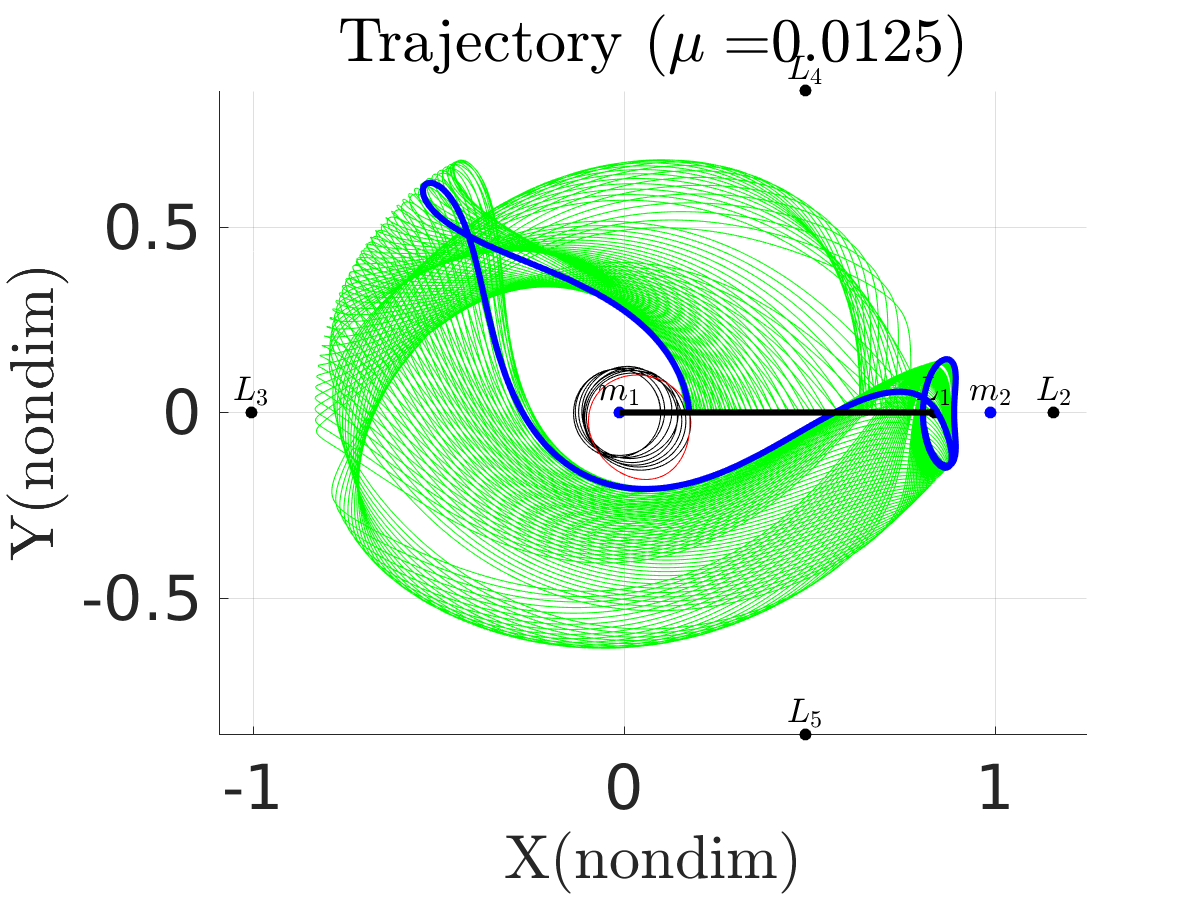
\includegraphics[width=0.45\textwidth]{figures/2017_JAS/geo_transfer_full}}\hfill
        \subcaptionbox{Detailed view of transfer: Centered at \(m_1\) the eight
            iterations from the reachability analysis are shown in black.  The
            final segment to the stable manifold is shown in red.  Each
            iteration progressively approaches the stable manifold.  Once on
        the stable manifold the vehicle can coast without thrust towards the
    periodic orbit.\label{fig:geo_transfer_zoom}
}{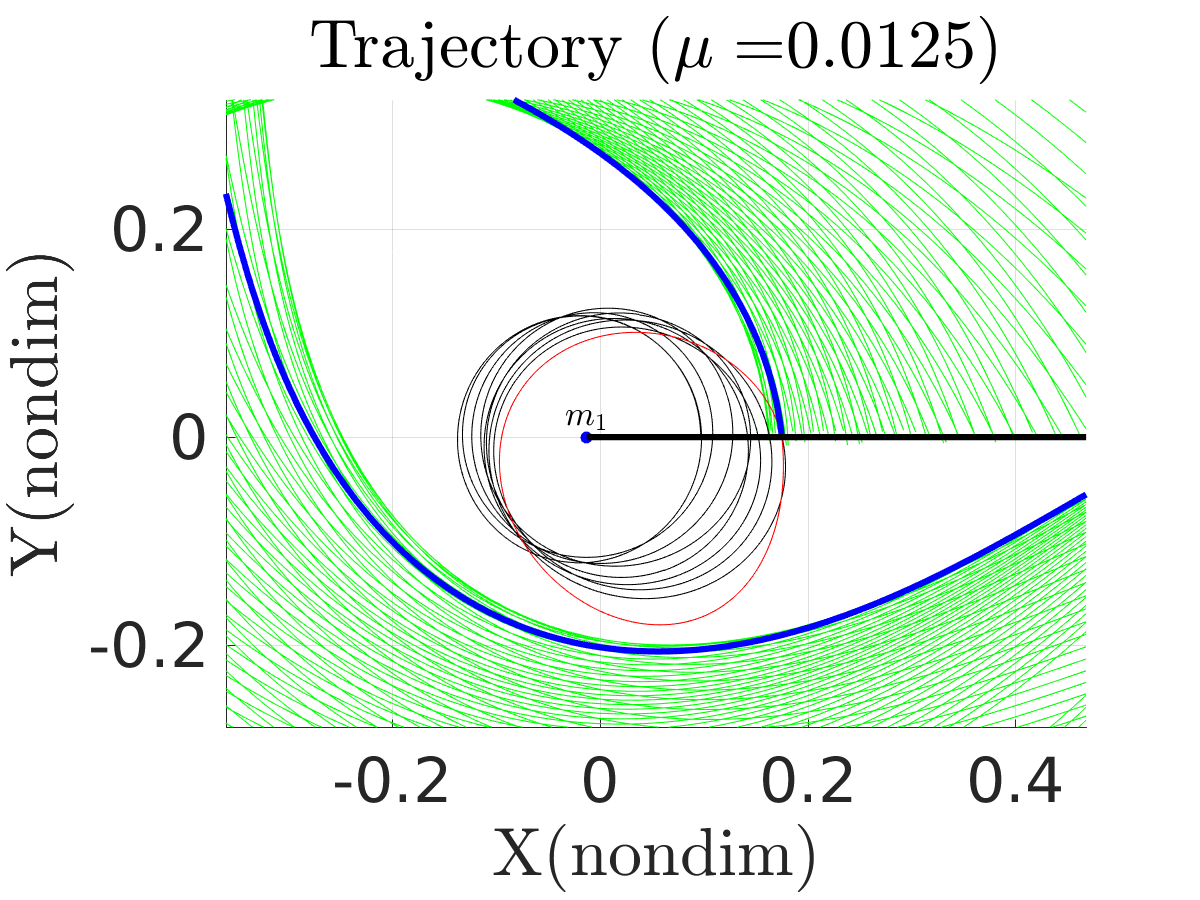
\includegraphics[width=0.45\textwidth]{figures/2017_JAS/geo_transfer_zoom}}
       
\subcaptionbox{\Poincare section: Minimum distance states from each iteration of the reachability set analysis (red) with respect to the stable invariant manifold (green)\label{fig:geo_transfer_poincare}}{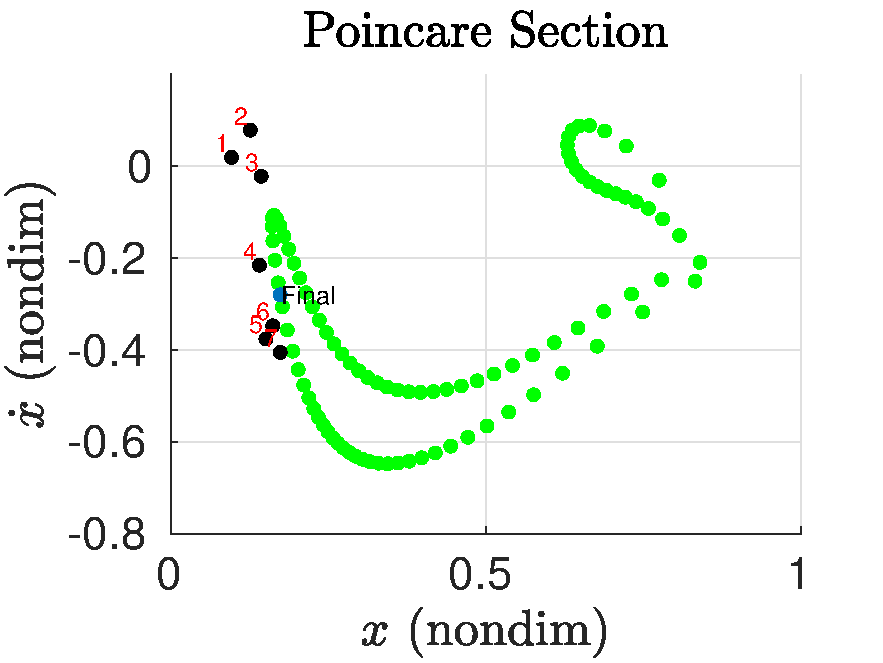
\includegraphics[width=0.45\textwidth]{figures/2017_JAS/poincare}}
    \hfill
    \subcaptionbox{Control Input: Combined control history for each stage of the reachability analysis. 
    The control always remains within the maximum bound.\label{fig:control_input_geo}}{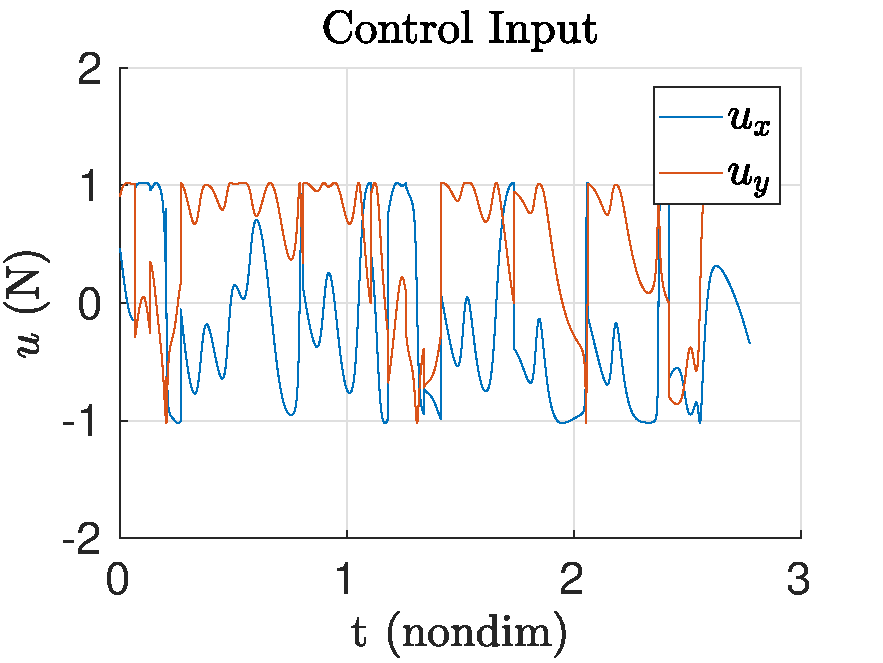
\includegraphics[width=0.45\textwidth]{figures/2017_JAS/control_input_geo.pdf}}

    \subcaptionbox{Jacobi Energy: Energy history throughout the transfer.
    Each stage of the transfer serves to increase the energy towards the stable manifold. 
The final reachability set intersects the stable manifold and enables a large final maneuver to the target orbit.\label{fig:jacobi_geo}}{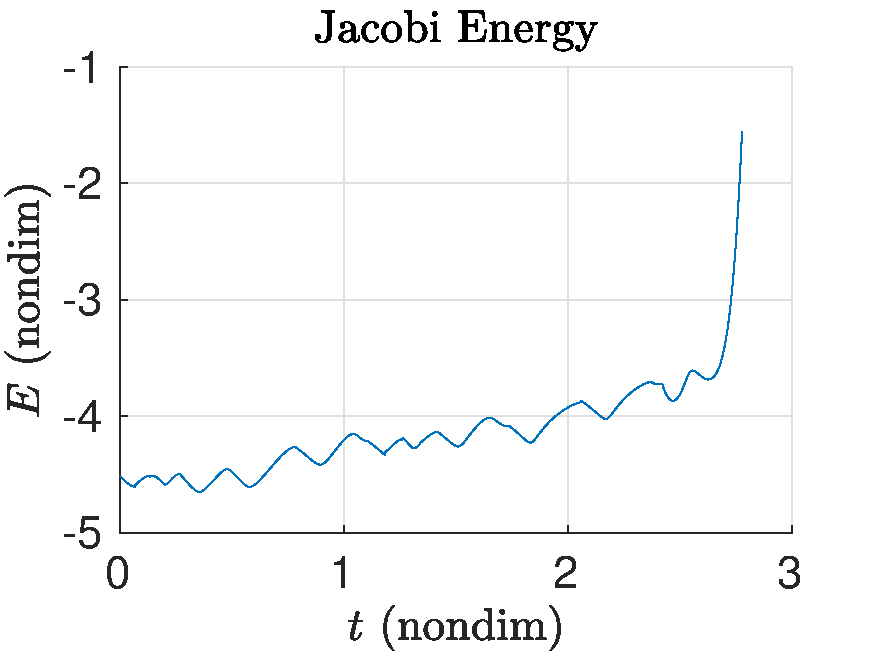
\includegraphics[width=0.5\textwidth]{figures/2017_JAS/jacobi_energy.pdf}}

        \caption{Geostationary to \( L_1 \) periodic orbit transfer: Complete transfer from the geostationary orbit to the stable manifold.\label{fig:geo_transfer}}
\end{figure}

This numerical example demonstrates the ability to link several computations of the reachability set to enable a more general transfer.
We use eight iterations of computing the reachability set in order to transfer from the geostationary orbit to the stable manifold.
This approach allows for a larger class of potential transfers which leverage the capabilities of low-thrust propulsion systems.
We are able to achieve a transfer that is not possible via the standard invariant manifold approach. 
In addition, this example illustrates a straightforward method to depart from the natural dynamics and transfer to a large region of the phase space that is not accessible via invariant manifolds alone.
\subsection{4769 Castalia Examples}
In this section, we extend the results developed in the planar three body problem to the higher dimensional space around an asteroid.
As shown in~\cref{sec:sc_eoms}, the translational dynamics of a point mass around an asteroid asteroid are similar to that of the three body problem.
Similar to~\cref{sec:periodic_orbit_transfer}, a \Poincare section is defined and the reachability set is approximated on this space. 
This lower dimensional space is used to design a transfer trajectory to move the vehicle between equatorial orbits of asteroid Castalia.

We apply the \Poincare map with a surface of section chosen to be normal to the position \( y = 0 \).
The \Poincare map is then defined as the map between successive transversal crossings of the surface of section.
To ensure a transverse crossing of the section we also require that \( \dot{y} \neq 0 \) when \( y = 0 \).
With this definition of the \Poincare map, it is possible to remove the two variables \( y \) and \( \dot{y} \) from consideration and create a four-dimensional map from the \Poincare section to itself.
The \Poincare section, represented by \( \Sigma \), then becomes
\begin{align}\label{eq:poincare_section}
    \Sigma = \braces{\parenth{x, \dot{x}, z, \dot{z}} | y(t_f) = 0 }.
\end{align}
We use this section to compute periodic orbits that serve as the initial and target states of our transfer.
In addition, this section serves as a lower dimensional space upon which we approximate the reachability set.

The cost function is given by~\cref{eq:cost}, but modified for the extra dimensions in this problem.
We use the matrix \( Q = \text{diag} \bracket{1~\>0~\> 1~\> 1~\>0~\>1 } \in \R^{6 \times 6}\) to represent the mapping onto \( \Sigma \).
Maximization of the distance between \( \vc{x}_n \) and \(\vc{x} \), on the \Poincare section defined in~\cref{eq:poincare_section}, is equivalent to the minimization of \( J \) defined in~\cref{eq:cost}.
We ensure that the trajectories intersect the \Poincare section through the use of terminal constraints.
In addition, we use the terminal constraints to define a specific direction along which we seek to minimize the cost~\cref{eq:cost}.
Since the \Poincare section is four-dimensional, we parameterize a direction in \( \R^4 \)  using three angles \( \phi_1, \phi_2 , \phi_3 \).
The terminal constraints are given in terms of these angles as
\begin{align}\label{eq:terminal_constraints}
    \begin{split}
        m_1 &= y = 0 , \\
        m_2 &= \parenth{\sin \phi_{1_{d}}} \parenth{ x_1^2 + x_2^2 + x_3^2 + x_4^2} - x_1^2 = 0, \\
        m_3 &= \parenth{\sin \phi_{2_{d}}} \parenth{ x_2^2 + x_3^2 + x_4^2} - x_2^2 = 0, \\
        m_4 &= \parenth{\sin \phi_{3_{d}}} \parenth{ 2 x_3^2 + 2 x_3 \sqrt{x_4^2 + 2 x_4^2}} - x_3 - \sqrt{x_4^2 + x_3^2} = 0 ,
    \end{split}
\end{align}
where we make use of the difference states \( \parenth{x_1, x_2 ,x_3, x_4 }\) defined as
\begin{align}\label{eq:diff_states}
    \begin{split}
        x_1 &= x(t_f) - x_n(t_f) , \\
        x_2 &= z(t_f) - z_n(t_f) , \\
        x_3 &= \dot{x}(t_f) - \dot{x}_n(t_f) , \\
        x_4 &= \dot{z}(t_f) - \dot{z}_n(t_f) . \\
    \end{split}
\end{align}
We select the terminal time, \( t_f \), from the time required for the uncontrolled trajectory to return back to the \Poincare section.
The constraint \( m_1 = 0 \) ensures that the terminal state lies on the \Poincare section.
The constraints \( m_2, m_3, m_4 \) are used to define a direction on the \Poincare section.
\Cref{eq:diff_states} represents the difference between our controlled and uncontrolled trajectory on the \Poincare section.
We approximate the entire reachable set by discretization  over the space of angles \(\phi_1, \phi_2, \phi_3 \).
By convention we assume that the angles lie in the following range
\begin{align*}
    \phi_1, \phi_2 &\in [ 0, \pi ) ,\\
    \phi_3 &\in [ 0 , 2 \pi ) ,
\end{align*}
such that we parameterize all directions on the three sphere, \(\S^3\).
Finally, we also incorporate the control acceleration magnitude constraint as
\begin{align}\label{eq:control_constraint}
    c(\vc{u}) = \vc{u}^T \vc{u} - u_m^2 \leq 0 ,
\end{align}
where \( u_m \) is the maximum acceleration possible by the propulsion system.
This constraint assumes that the control acceleration may be orientated in any direction yet the acceleration magnitude is variable but bounded.
The goal is to determine the control history \( \vc{u}(t) \) such that the cost function~\cref{eq:cost} is minimized while subject to the equations of motion~\cref{eq:body_eoms} and the constraints~\cref{eq:control_constraint,eq:terminal_constraints}.

We present an example transfer of a spacecraft about the asteroid 4769 Castalia. 
Our equations of motion, given by~\cref{eq:eoms}, are an idealized version of the dynamics of a spacecraft.
For example, the model does not include the effect of mass transfer from propellant usage. 
We instead model the control input as a generic acceleration vector in the body-fixed asteroid frame. 
The acceleration magnitude constraint in~\cref{eq:control_constraint} is chosen to emulate a physically realizable thruster system.
In this analysis, we assume \( u_m = \SI{0.1}{\milli\meter\per\second\squared}\) which is equivalent to a thrust of approximately \SI{100}{\milli\newton} for a \SI{1000}{\kilo\gram} spacecraft.
This amount of thrust is typical of many current ion or hall effect thrusters~\cite{goebel2008,choueiri2009}.

The objective is to transfer the spacecraft between two periodic equatorial orbits about Castalia.
The initial and target orbits are periodic solutions about Castlia computed using the method introduced by Reference~\cite{scheeres2003}.
The initial conditions for both orbits are defined in the body-fixed frame as
\begin{align}\label{sec:initial_transfer}
    \vc{x}_i = 
    \begin{bmatrix}
        1.4973 \\ 0 \\ 0.0061 \\ 0\\ -0.0009 \\ 0
    \end{bmatrix} ,
    \quad
    \vc{x}_t =
    \begin{bmatrix}
        6.1175 \\ 0 \\ 0.0001 \\ 0\\ -0.0025 \\ 0
    \end{bmatrix} .
\end{align}
\Cref{fig:initial_transfer} shows the initial, \( \vc{x}_i \), and target, \( \vc{x}_t\), periodic orbits which lie in the equatorial plane of Castalia.
Our goal is to transfer from a lower altitude to a higher altitude while remaining in the equatorial plane of the asteroid.
This type of scenario would occur frequently during mapping and observation missions to asteroids.
\begin{figure}[htbp]
    \centering 
    \begin{subfigure}[htbp]{0.45\textwidth} 
        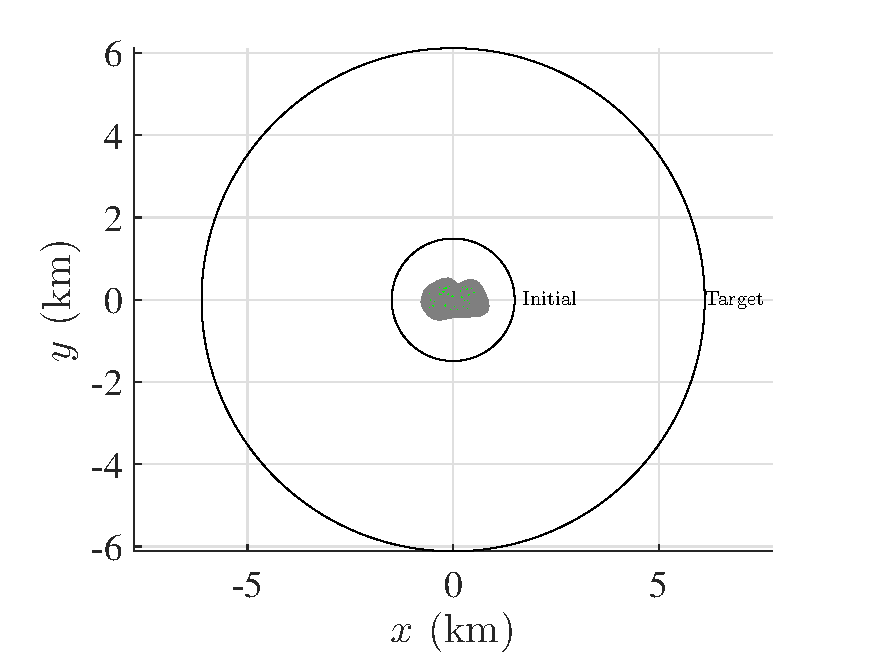
\includegraphics[width=\textwidth]{figures/2016_AAS/initial_transfer} 
        \caption{Equatorial View} \label{fig:eq_initial_transfer} 
    \end{subfigure}~ %add desired spacing between images, e. g. ~, \quad, \qquad, \hfill etc. %(or a blank line to force the subfigure onto a new line) 
    \begin{subfigure}[htbp]{0.45\textwidth} 
        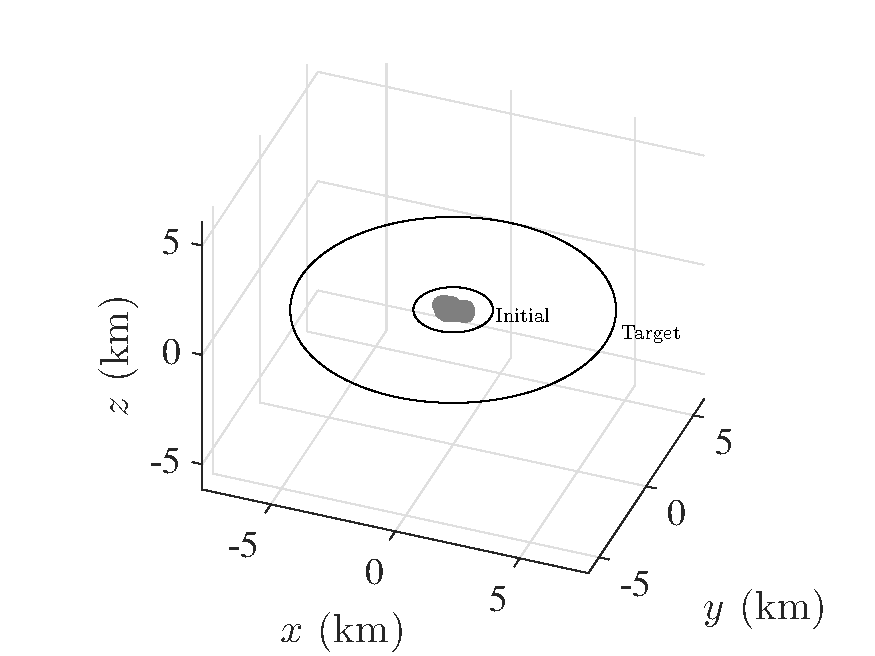
\includegraphics[width=\textwidth]{figures/2016_AAS/initial_transfer_3d} 
        \caption{3D view} \label{fig:initial_transfer_3d} 
    \end{subfigure} ~ %add desired spacing between images, e. g. ~, \quad, \qquad, \hfill etc. %(or a blank line to force the subfigure onto a new line) 
    \caption{Initial and target periodic orbits}
    \label{fig:initial_transfer} 
\end{figure}
In this transfer example we also have used a reduced model of Castalia.
Rather than using the full \num{4092} face model we reduce the number of faces to \num{1024} using the Matlab function \verb+reducepatch+. 
This greatly speeds up the computation with only a small difference in the gravitational field.

We first compute the reachability set originating from the initial periodic orbit at \( \vecbf{x}_i\) for a fixed time of flight and bounded control magnitude as defined previously.
The reachability set is computed by solving the two-point boundary value problem using a multiple shooting algorithm to satisfy the necessary conditions in~\cref{eq:necc_conditions}.
The reachability set is generated on the lower dimensional \Poincare section and is composed of the terminal states in the \( \parenth{x,z,\dot{x},\dot{z} } \) space.
We approximate the reachability set by discretization of each of the angles \( \phi_1, \phi_2 , \phi_3 \) into ten discrete steps. 
This results in a total of \(10^3\) trajectories which approximate the reachability set on the \Poincare section.

We visualize the section using the two figures in~\cref{fig:poincare_section}.
\begin{figure}[htbp]
    \centering 
    \begin{subfigure}[htbp]{0.45\textwidth} 
        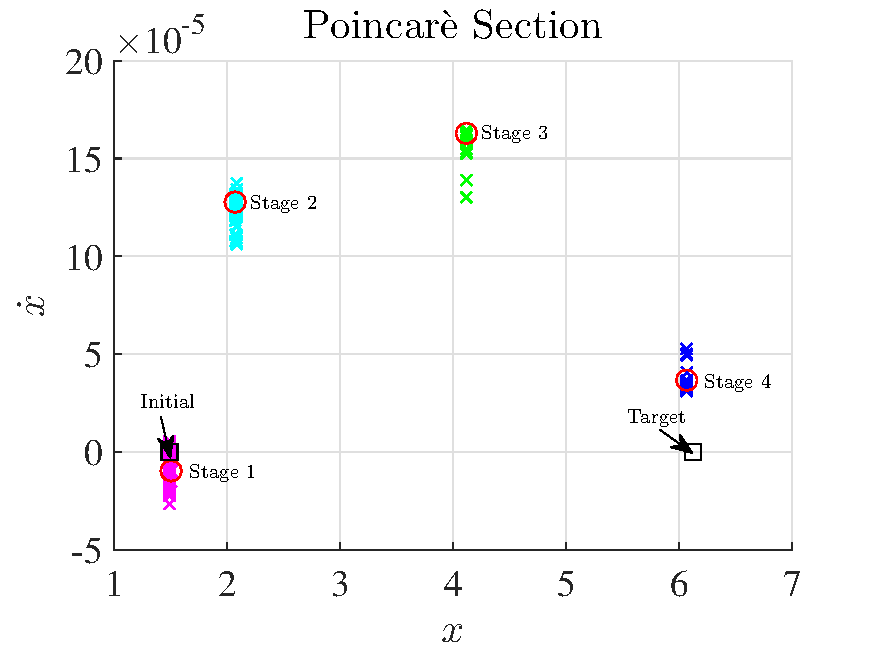
\includegraphics[width=\textwidth]{figures/2016_AAS/poincare_xvsxdot.pdf} 
        \caption{\( x \) vs. \( \dot{x} \) \Poincare section} \label{fig:poincare_xvsxdot} 
    \end{subfigure}~
    \begin{subfigure}[htbp]{0.45\textwidth} 
        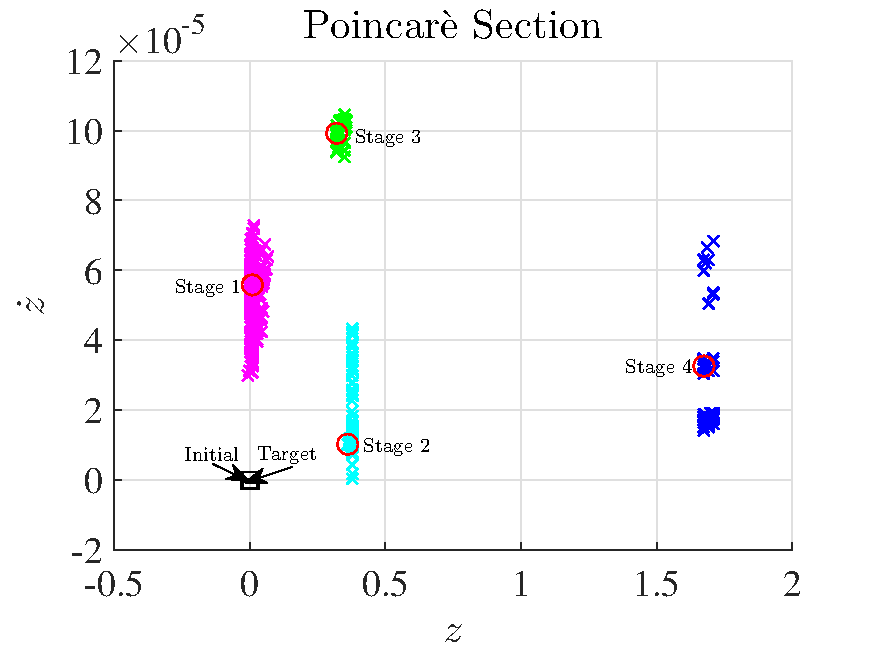
\includegraphics[width=\textwidth]{figures/2016_AAS/poincare_zvszdot.pdf} 
        \caption{\( z \) vs. \( \dot{z} \) \Poincare section} \label{fig:poincare_zvszdot} 
    \end{subfigure}
    \caption{\Poincare section visualization \label{fig:poincare_section}}
\end{figure}
These two-dimensional sections allow us to visualize the four-dimensional \Poincare section defined by~\cref{eq:poincare_section}.
The first stage of the transfer is represented by the magenta markers in~\cref{fig:poincare_section}.
From~\cref{fig:poincare_xvsxdot}, we can see that the reachability set has grown in the \( \dot{x} \) dimension but has not been enlarged much in the \( x \) direction.
Similarly,~\cref{fig:poincare_zvszdot} shows an increase in the \( \dot{z} \) component.
From the reachability set, we chose a trajectory and terminal state which minimizes a distance metric \( d(\vecbf{x}_f,\vecbf{x}_t) \) to the desired target
\begin{align}\label{eq:reach_dist}
    d = \sqrt{k_x \parenth{x_f - x_t }^2 + k_z \parenth{z_f - z_t }^2 + k_{\dot{x}}\parenth{\dot{x}_f - \dot{x}_t }^2 + k_{\dot{z}}\parenth{\dot{z}_f - \dot{z}_t }^2} ,
\end{align}
where \( k_x, k_z, k_{\dot{x}}, k_{\dot{z}} \) are used to weight the relative importance of each of the components of the \Poincare section.
\Cref{fig:phi_distance} shows the distance to the target for the chosen discretization of \( \phi_i \).
\begin{figure}[htbp] 
    \centering 
    \begin{subfigure}[htbp]{0.3\textwidth} 
        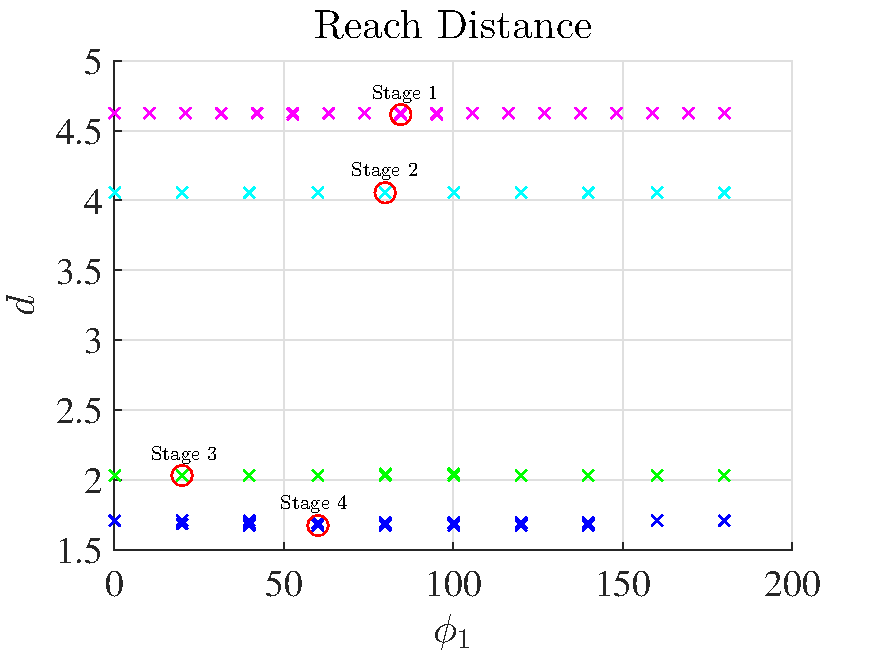
\includegraphics[width=\textwidth]{figures/2016_AAS/phi1.pdf} 
        \caption{ \( \phi_1 \)} \label{fig:phi1} 
    \end{subfigure}~
    \begin{subfigure}[htbp]{0.3\textwidth} 
        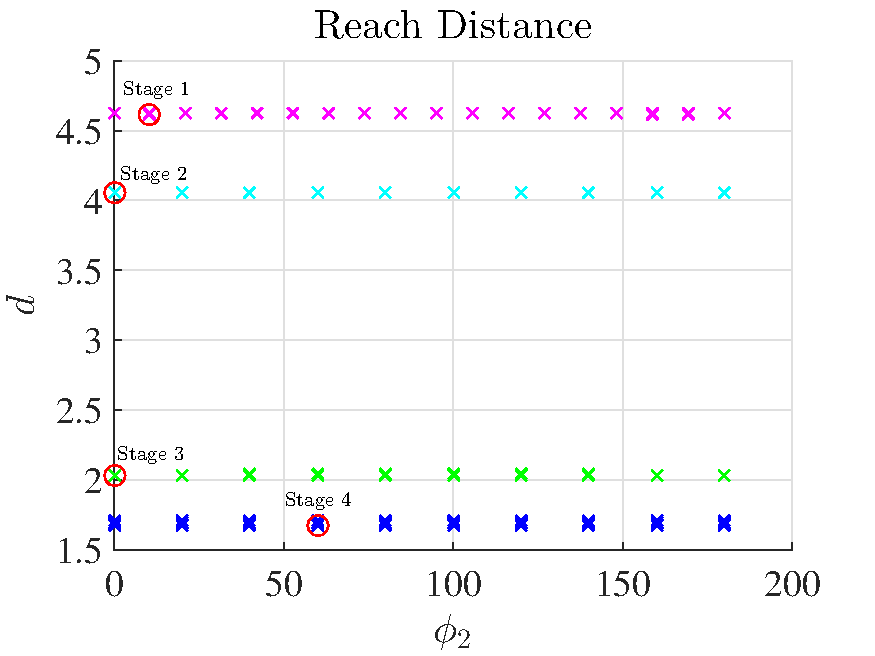
\includegraphics[width=\textwidth]{figures/2016_AAS/phi2.pdf} 
        \caption{\( \phi_2 \)} \label{fig:phi2} 
    \end{subfigure}~
    \begin{subfigure}[htbp]{0.3\textwidth} 
        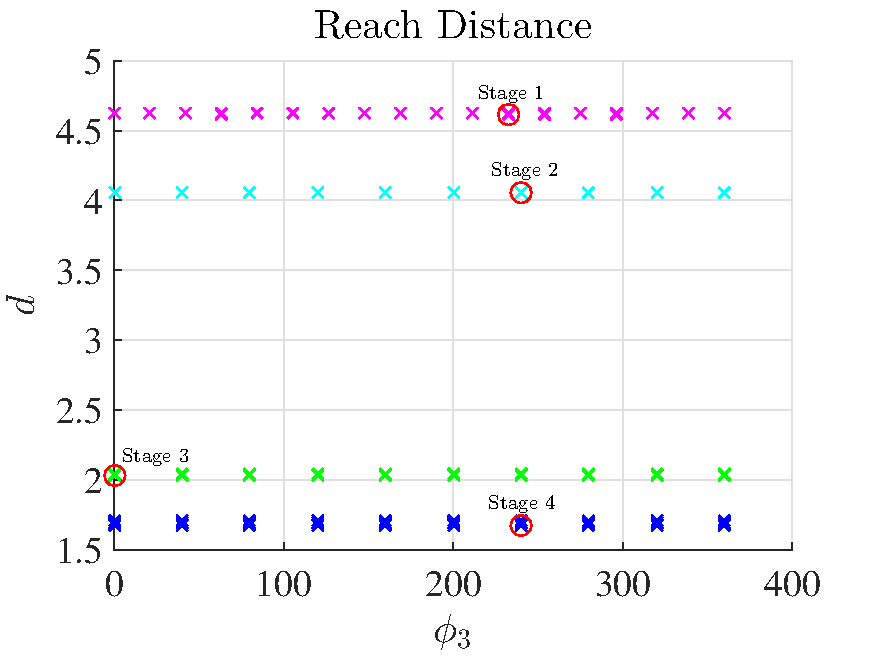
\includegraphics[width=\textwidth]{figures/2016_AAS/phi3.pdf} 
        \caption{\( \phi_3 \)} \label{fig:phi3} 
    \end{subfigure} 
    \caption{Variation of \(d(\vecbf{x}_f,\vecbf{x}_t)\) due to \( \phi_i\)}
    \label{fig:phi_distance} 
\end{figure}

The trajectory which minimizes \( d \) is indicated by the red circular markers in~\cref{fig:poincare_section,fig:phi_distance}.
Since the first reachability set does not include the target we use the minimum state from the first stage to initialize another reachability computation.
Once again we compute the reachability set by discretization of the angles \( \phi_i \) on the \Poincare section.
This second stage, represented by the cyan markers in~\cref{fig:poincare_section,fig:phi_distance}, further increases the \( x, z\) components but does not reach the target orbit.
As a result, a third and forth stage are generated in a similar manner and shown by the green and blue markers in~\cref{fig:poincare_section,fig:phi_distance}, respectively.
We can see in~\cref{fig:poincare_section} that the reachability set of the forth stage includes both the \( x \) and \( z\) components of the target periodic orbit.
At the same time there is a relatively large difference between the \( \dot{x} \), \( \dot{z} \), and \( z \) components of the forth stage and the target orbit.
In practice, this is not a large concern as we have direct control over the spacecraft velocity via the control input and the equatorial plane still remains within the reachability set of the transfer.

With the reachability set encompassing the target orbit, we can generate a final transfer to the target.
We use the minimum state calculated from the final stage to serve as the initial condition of the transfer.
A final optimal transfer is computed to satisfy the fixed terminal state \( \vc{x}(t_f) = \vc{x}_t \) and the bounded control magnitude constraint.
\Cref{fig:trajectory} shows the entire transfer trajectory, from the four reachable set trajectories as well as the final transfer to the target.
\begin{figure}[htbp] 
    \centering 
    \begin{subfigure}[htbp]{0.45\textwidth} 
        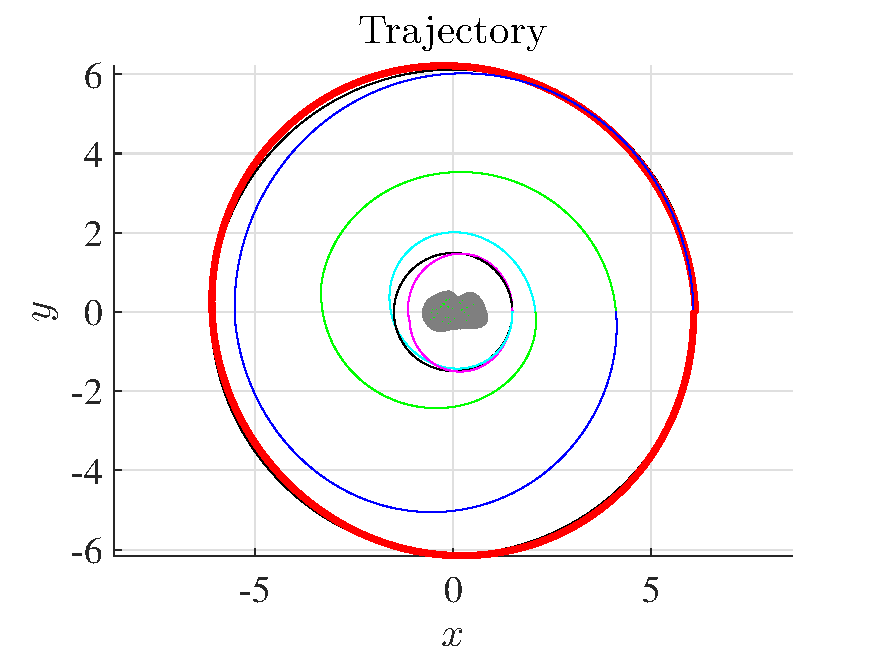
\includegraphics[width=\textwidth]{figures/2016_AAS/trajectory.pdf} 
        \caption{Equatorial view of transfer} \label{fig:trajectory_up} 
    \end{subfigure}~
    \begin{subfigure}[htbp]{0.45\textwidth} 
        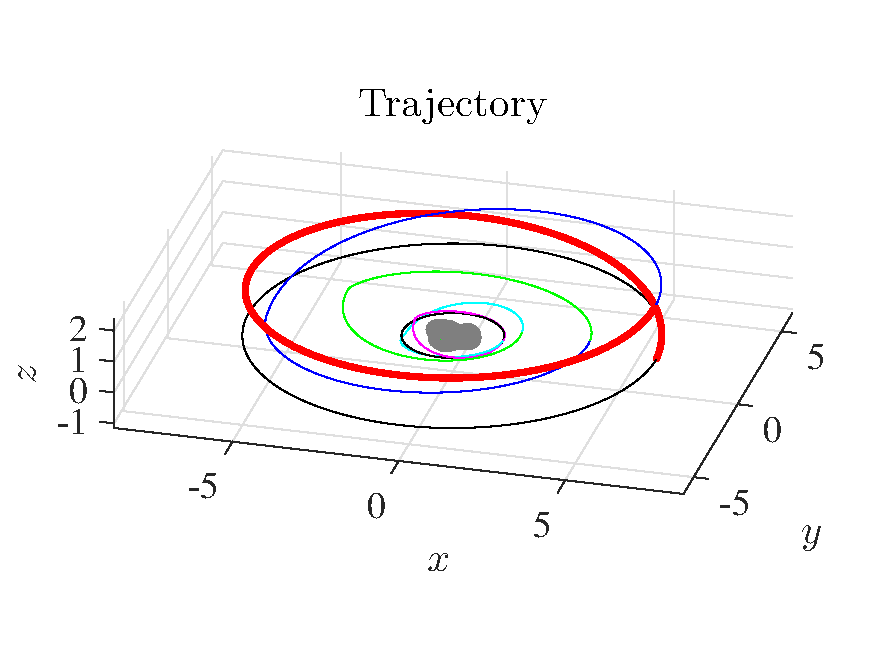
\includegraphics[width=\textwidth]{figures/2016_AAS/trajectory_3d.pdf} 
        \caption{Out of plane view} \label{fig:trajectory_3d} 
    \end{subfigure}~ 
    \caption{Complete transfer trajectory}
    \label{fig:trajectory} 
\end{figure}
It is interesting to note that while both the initial and target periodic orbit lie in the equatorial plane, the reachability trajectories show a relatively large out of plane component during the transfers.
In spite of this out of plane movement, the reachability set approaches and meets the target orbit. 
\begin{figure}
    \centering
    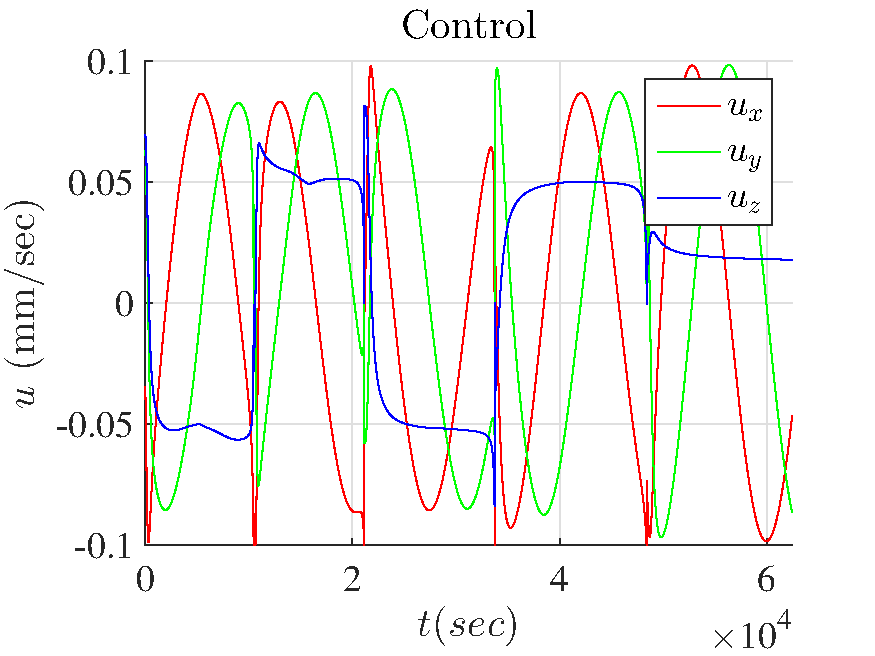
\includegraphics[width=0.45\textwidth]{figures/2016_AAS/control.pdf}
    \caption{Control history \label{fig:control}}
\end{figure}
\Cref{fig:control} shows the control input required during the maneuver.
We can see that the control constraint in~\cref{eq:control_constraint} is satisfied over the entire trajectory.
